\documentclass[english]{article}
\usepackage[utf8]{inputenc}
\usepackage[T1]{fontenc}
\usepackage{babel}
\usepackage{comment}
\usepackage{svg}
\usepackage{caption, booktabs}
\usepackage{amsmath}
\usepackage{graphicx}
\usepackage{fancyhdr}
% \usepackage[disable]{todonotes}
\usepackage{todonotes}
\usepackage{units}
\usepackage[left=2cm,right=4cm,top=2cm,bottom=2cm]{geometry}
\usepackage[
	colorlinks=true,
	citecolor=black,
  urlcolor=black,
	linkcolor=black
]{hyperref}
\newcommand{\scidatalogo}{
\includegraphics[height=36pt]{SciData_logo.jpg}}
\pagestyle{fancy}
\fancyhf{}
\renewcommand{\headrulewidth}{0pt}
\setlength{\headheight}{40pt}
\lhead{\textsc{\scidatalogo}}
\usepackage{natbib}

\begin{document}
\newcommand{\aoBodyAll}{66}
\newcommand{\aoBodyI}{6}
\newcommand{\aoBodyII}{12}
\newcommand{\aoBodyIII}{7}
\newcommand{\aoBodyIV}{12}
\newcommand{\aoBodyV}{2}
\newcommand{\aoBodyVI}{9}
\newcommand{\aoBodyVII}{13}
\newcommand{\aoBodyVIII}{5}

\newcommand{\aoBpartAll}{69}
\newcommand{\aoBpartI}{9}
\newcommand{\aoBpartII}{8}
\newcommand{\aoBpartIII}{6}
\newcommand{\aoBpartIV}{13}
\newcommand{\aoBpartV}{5}
\newcommand{\aoBpartVI}{7}
\newcommand{\aoBpartVII}{11}
\newcommand{\aoBpartVIII}{10}

\newcommand{\aoFaheadAll}{83}
\newcommand{\aoFaheadI}{12}
\newcommand{\aoFaheadII}{11}
\newcommand{\aoFaheadIII}{10}
\newcommand{\aoFaheadIV}{5}
\newcommand{\aoFaheadV}{9}
\newcommand{\aoFaheadVI}{13}
\newcommand{\aoFaheadVII}{12}
\newcommand{\aoFaheadVIII}{11}

\newcommand{\aoFgadlrdiffAll}{180133}
\newcommand{\aoFgadlrdiffI}{22574}
\newcommand{\aoFgadlrdiffII}{22075}
\newcommand{\aoFgadlrdiffIII}{21925}
\newcommand{\aoFgadlrdiffIV}{24425}
\newcommand{\aoFgadlrdiffV}{23125}
\newcommand{\aoFgadlrdiffVI}{21975}
\newcommand{\aoFgadlrdiffVII}{27175}
\newcommand{\aoFgadlrdiffVIII}{16859}

\newcommand{\aoFgadrmsAll}{180133}
\newcommand{\aoFgadrmsI}{22574}
\newcommand{\aoFgadrmsII}{22075}
\newcommand{\aoFgadrmsIII}{21925}
\newcommand{\aoFgadrmsIV}{24425}
\newcommand{\aoFgadrmsV}{23125}
\newcommand{\aoFgadrmsVI}{21975}
\newcommand{\aoFgadrmsVII}{27175}
\newcommand{\aoFgadrmsVIII}{16859}

\newcommand{\aoFurnAll}{50}
\newcommand{\aoFurnI}{8}
\newcommand{\aoFurnII}{5}
\newcommand{\aoFurnIII}{2}
\newcommand{\aoFurnIV}{5}
\newcommand{\aoFurnV}{7}
\newcommand{\aoFurnVI}{10}
\newcommand{\aoFurnVII}{7}
\newcommand{\aoFurnVIII}{6}

\newcommand{\aoGeoAll}{125}
\newcommand{\aoGeoI}{16}
\newcommand{\aoGeoII}{17}
\newcommand{\aoGeoIII}{11}
\newcommand{\aoGeoIV}{32}
\newcommand{\aoGeoV}{0}
\newcommand{\aoGeoVI}{15}
\newcommand{\aoGeoVII}{18}
\newcommand{\aoGeoVIII}{16}

\newcommand{\aoGroomAll}{105}
\newcommand{\aoGroomI}{12}
\newcommand{\aoGroomII}{11}
\newcommand{\aoGroomIII}{8}
\newcommand{\aoGroomIV}{5}
\newcommand{\aoGroomV}{8}
\newcommand{\aoGroomVI}{25}
\newcommand{\aoGroomVII}{28}
\newcommand{\aoGroomVIII}{8}

\newcommand{\aoObjAll}{284}
\newcommand{\aoObjI}{39}
\newcommand{\aoObjII}{34}
\newcommand{\aoObjIII}{27}
\newcommand{\aoObjIV}{44}
\newcommand{\aoObjV}{29}
\newcommand{\aoObjVI}{42}
\newcommand{\aoObjVII}{32}
\newcommand{\aoObjVIII}{37}

\newcommand{\aoSenewAll}{86}
\newcommand{\aoSenewI}{11}
\newcommand{\aoSenewII}{15}
\newcommand{\aoSenewIII}{12}
\newcommand{\aoSenewIV}{4}
\newcommand{\aoSenewV}{15}
\newcommand{\aoSenewVI}{10}
\newcommand{\aoSenewVII}{16}
\newcommand{\aoSenewVIII}{3}

\newcommand{\aoSeoldAll}{37}
\newcommand{\aoSeoldI}{2}
\newcommand{\aoSeoldII}{5}
\newcommand{\aoSeoldIII}{1}
\newcommand{\aoSeoldIV}{4}
\newcommand{\aoSeoldV}{2}
\newcommand{\aoSeoldVI}{9}
\newcommand{\aoSeoldVII}{8}
\newcommand{\aoSeoldVIII}{6}

\newcommand{\aoSexfAll}{108}
\newcommand{\aoSexfI}{14}
\newcommand{\aoSexfII}{22}
\newcommand{\aoSexfIII}{6}
\newcommand{\aoSexfIV}{6}
\newcommand{\aoSexfV}{13}
\newcommand{\aoSexfVI}{10}
\newcommand{\aoSexfVII}{23}
\newcommand{\aoSexfVIII}{14}

\newcommand{\aoSexmAll}{403}
\newcommand{\aoSexmI}{41}
\newcommand{\aoSexmII}{68}
\newcommand{\aoSexmIII}{38}
\newcommand{\aoSexmIV}{102}
\newcommand{\aoSexmV}{45}
\newcommand{\aoSexmVI}{42}
\newcommand{\aoSexmVII}{42}
\newcommand{\aoSexmVIII}{25}

\newcommand{\aoSexuAll}{17}
\newcommand{\aoSexuI}{0}
\newcommand{\aoSexuII}{3}
\newcommand{\aoSexuIII}{1}
\newcommand{\aoSexuIV}{2}
\newcommand{\aoSexuV}{3}
\newcommand{\aoSexuVI}{1}
\newcommand{\aoSexuVII}{5}
\newcommand{\aoSexuVIII}{2}

\newcommand{\aoVlochAll}{89}
\newcommand{\aoVlochI}{10}
\newcommand{\aoVlochII}{31}
\newcommand{\aoVlochIII}{2}
\newcommand{\aoVlochIV}{23}
\newcommand{\aoVlochV}{4}
\newcommand{\aoVlochVI}{18}
\newcommand{\aoVlochVII}{1}
\newcommand{\aoVnocutAll}{148}
\newcommand{\aoVnocutI}{30}
\newcommand{\aoVnocutII}{13}
\newcommand{\aoVnocutIII}{21}
\newcommand{\aoVnocutIV}{15}
\newcommand{\aoVnocutV}{27}
\newcommand{\aoVnocutVI}{9}
\newcommand{\aoVnocutVII}{17}
\newcommand{\aoVnocutVIII}{16}

\newcommand{\aoVpenewAll}{386}
\newcommand{\aoVpenewI}{31}
\newcommand{\aoVpenewII}{38}
\newcommand{\aoVpenewIII}{72}
\newcommand{\aoVpenewIV}{90}
\newcommand{\aoVpenewV}{89}
\newcommand{\aoVpenewVI}{33}
\newcommand{\aoVpenewVII}{24}
\newcommand{\aoVpenewVIII}{9}

\newcommand{\aoVpeoldAll}{208}
\newcommand{\aoVpeoldI}{25}
\newcommand{\aoVpeoldII}{61}
\newcommand{\aoVpeoldIII}{13}
\newcommand{\aoVpeoldIV}{1}
\newcommand{\aoVpeoldV}{32}
\newcommand{\aoVpeoldVI}{29}
\newcommand{\aoVpeoldVII}{47}
\newcommand{\aoVsenewAll}{96}
\newcommand{\aoVsenewI}{11}
\newcommand{\aoVsenewII}{14}
\newcommand{\aoVsenewIII}{17}
\newcommand{\aoVsenewIV}{4}
\newcommand{\aoVsenewV}{17}
\newcommand{\aoVsenewVI}{9}
\newcommand{\aoVsenewVII}{21}
\newcommand{\aoVsenewVIII}{3}

\newcommand{\aoVseoldAll}{90}
\newcommand{\aoVseoldI}{7}
\newcommand{\aoVseoldII}{11}
\newcommand{\aoVseoldIII}{3}
\newcommand{\aoVseoldIV}{7}
\newcommand{\aoVseoldV}{7}
\newcommand{\aoVseoldVI}{23}
\newcommand{\aoVseoldVII}{15}
\newcommand{\aoVseoldVIII}{17}


\newcommand{\avBodyAll}{66}
\newcommand{\avBodyI}{6}
\newcommand{\avBodyII}{12}
\newcommand{\avBodyIII}{7}
\newcommand{\avBodyIV}{12}
\newcommand{\avBodyV}{2}
\newcommand{\avBodyVI}{9}
\newcommand{\avBodyVII}{13}
\newcommand{\avBodyVIII}{5}

\newcommand{\avBpartAll}{69}
\newcommand{\avBpartI}{9}
\newcommand{\avBpartII}{8}
\newcommand{\avBpartIII}{6}
\newcommand{\avBpartIV}{13}
\newcommand{\avBpartV}{5}
\newcommand{\avBpartVI}{7}
\newcommand{\avBpartVII}{11}
\newcommand{\avBpartVIII}{10}

\newcommand{\avFaheadAll}{83}
\newcommand{\avFaheadI}{12}
\newcommand{\avFaheadII}{11}
\newcommand{\avFaheadIII}{10}
\newcommand{\avFaheadIV}{5}
\newcommand{\avFaheadV}{9}
\newcommand{\avFaheadVI}{13}
\newcommand{\avFaheadVII}{12}
\newcommand{\avFaheadVIII}{11}

\newcommand{\avFgavgerlrAll}{180783}
\newcommand{\avFgavgerlrI}{22656}
\newcommand{\avFgavgerlrII}{22158}
\newcommand{\avFgavgerlrIII}{22008}
\newcommand{\avFgavgerlrIV}{24507}
\newcommand{\avFgavgerlrV}{23208}
\newcommand{\avFgavgerlrVI}{22057}
\newcommand{\avFgavgerlrVII}{27208}
\newcommand{\avFgavgerlrVIII}{16981}

\newcommand{\avFgavgerlrdiffAll}{180759}
\newcommand{\avFgavgerlrdiffI}{22653}
\newcommand{\avFgavgerlrdiffII}{22155}
\newcommand{\avFgavgerlrdiffIII}{22005}
\newcommand{\avFgavgerlrdiffIV}{24504}
\newcommand{\avFgavgerlrdiffV}{23205}
\newcommand{\avFgavgerlrdiffVI}{22054}
\newcommand{\avFgavgerlrdiffVII}{27205}
\newcommand{\avFgavgerlrdiffVIII}{16978}

\newcommand{\avFgavgermlAll}{180783}
\newcommand{\avFgavgermlI}{22656}
\newcommand{\avFgavgermlII}{22158}
\newcommand{\avFgavgermlIII}{22008}
\newcommand{\avFgavgermlIV}{24507}
\newcommand{\avFgavgermlV}{23208}
\newcommand{\avFgavgermlVI}{22057}
\newcommand{\avFgavgermlVII}{27208}
\newcommand{\avFgavgermlVIII}{16981}

\newcommand{\avFgavgerpdAll}{180783}
\newcommand{\avFgavgerpdI}{22656}
\newcommand{\avFgavgerpdII}{22158}
\newcommand{\avFgavgerpdIII}{22008}
\newcommand{\avFgavgerpdIV}{24507}
\newcommand{\avFgavgerpdV}{23208}
\newcommand{\avFgavgerpdVI}{22057}
\newcommand{\avFgavgerpdVII}{27208}
\newcommand{\avFgavgerpdVIII}{16981}

\newcommand{\avFgavgerrmsAll}{180759}
\newcommand{\avFgavgerrmsI}{22653}
\newcommand{\avFgavgerrmsII}{22155}
\newcommand{\avFgavgerrmsIII}{22005}
\newcommand{\avFgavgerrmsIV}{24504}
\newcommand{\avFgavgerrmsV}{23205}
\newcommand{\avFgavgerrmsVI}{22054}
\newcommand{\avFgavgerrmsVII}{27205}
\newcommand{\avFgavgerrmsVIII}{16978}

\newcommand{\avFgavgerudAll}{180783}
\newcommand{\avFgavgerudI}{22656}
\newcommand{\avFgavgerudII}{22158}
\newcommand{\avFgavgerudIII}{22008}
\newcommand{\avFgavgerudIV}{24507}
\newcommand{\avFgavgerudV}{23208}
\newcommand{\avFgavgerudVI}{22057}
\newcommand{\avFgavgerudVII}{27208}
\newcommand{\avFgavgerudVIII}{16981}

\newcommand{\avFurnAll}{50}
\newcommand{\avFurnI}{8}
\newcommand{\avFurnII}{5}
\newcommand{\avFurnIII}{2}
\newcommand{\avFurnIV}{5}
\newcommand{\avFurnV}{7}
\newcommand{\avFurnVI}{10}
\newcommand{\avFurnVII}{7}
\newcommand{\avFurnVIII}{6}

\newcommand{\avGeoAll}{125}
\newcommand{\avGeoI}{16}
\newcommand{\avGeoII}{17}
\newcommand{\avGeoIII}{11}
\newcommand{\avGeoIV}{32}
\newcommand{\avGeoV}{0}
\newcommand{\avGeoVI}{15}
\newcommand{\avGeoVII}{18}
\newcommand{\avGeoVIII}{16}

\newcommand{\avGroomAll}{105}
\newcommand{\avGroomI}{12}
\newcommand{\avGroomII}{11}
\newcommand{\avGroomIII}{8}
\newcommand{\avGroomIV}{5}
\newcommand{\avGroomV}{8}
\newcommand{\avGroomVI}{25}
\newcommand{\avGroomVII}{28}
\newcommand{\avGroomVIII}{8}

\newcommand{\avObjAll}{284}
\newcommand{\avObjI}{39}
\newcommand{\avObjII}{34}
\newcommand{\avObjIII}{27}
\newcommand{\avObjIV}{44}
\newcommand{\avObjV}{29}
\newcommand{\avObjVI}{42}
\newcommand{\avObjVII}{32}
\newcommand{\avObjVIII}{37}

\newcommand{\avSenewAll}{86}
\newcommand{\avSenewI}{11}
\newcommand{\avSenewII}{15}
\newcommand{\avSenewIII}{12}
\newcommand{\avSenewIV}{4}
\newcommand{\avSenewV}{15}
\newcommand{\avSenewVI}{10}
\newcommand{\avSenewVII}{16}
\newcommand{\avSenewVIII}{3}

\newcommand{\avSeoldAll}{37}
\newcommand{\avSeoldI}{2}
\newcommand{\avSeoldII}{5}
\newcommand{\avSeoldIII}{1}
\newcommand{\avSeoldIV}{4}
\newcommand{\avSeoldV}{2}
\newcommand{\avSeoldVI}{9}
\newcommand{\avSeoldVII}{8}
\newcommand{\avSeoldVIII}{6}

\newcommand{\avSexfAll}{108}
\newcommand{\avSexfI}{14}
\newcommand{\avSexfII}{22}
\newcommand{\avSexfIII}{6}
\newcommand{\avSexfIV}{6}
\newcommand{\avSexfV}{13}
\newcommand{\avSexfVI}{10}
\newcommand{\avSexfVII}{23}
\newcommand{\avSexfVIII}{14}

\newcommand{\avSexmAll}{403}
\newcommand{\avSexmI}{41}
\newcommand{\avSexmII}{68}
\newcommand{\avSexmIII}{38}
\newcommand{\avSexmIV}{102}
\newcommand{\avSexmV}{45}
\newcommand{\avSexmVI}{42}
\newcommand{\avSexmVII}{42}
\newcommand{\avSexmVIII}{25}

\newcommand{\avSexuAll}{17}
\newcommand{\avSexuI}{0}
\newcommand{\avSexuII}{3}
\newcommand{\avSexuIII}{1}
\newcommand{\avSexuIV}{2}
\newcommand{\avSexuV}{3}
\newcommand{\avSexuVI}{1}
\newcommand{\avSexuVII}{5}
\newcommand{\avSexuVIII}{2}

\newcommand{\avVlochAll}{89}
\newcommand{\avVlochI}{10}
\newcommand{\avVlochII}{31}
\newcommand{\avVlochIII}{2}
\newcommand{\avVlochIV}{23}
\newcommand{\avVlochV}{4}
\newcommand{\avVlochVI}{18}
\newcommand{\avVlochVII}{1}
\newcommand{\avVnocutAll}{148}
\newcommand{\avVnocutI}{30}
\newcommand{\avVnocutII}{13}
\newcommand{\avVnocutIII}{21}
\newcommand{\avVnocutIV}{15}
\newcommand{\avVnocutV}{27}
\newcommand{\avVnocutVI}{9}
\newcommand{\avVnocutVII}{17}
\newcommand{\avVnocutVIII}{16}

\newcommand{\avVpenewAll}{386}
\newcommand{\avVpenewI}{31}
\newcommand{\avVpenewII}{38}
\newcommand{\avVpenewIII}{72}
\newcommand{\avVpenewIV}{90}
\newcommand{\avVpenewV}{89}
\newcommand{\avVpenewVI}{33}
\newcommand{\avVpenewVII}{24}
\newcommand{\avVpenewVIII}{9}

\newcommand{\avVpeoldAll}{208}
\newcommand{\avVpeoldI}{25}
\newcommand{\avVpeoldII}{61}
\newcommand{\avVpeoldIII}{13}
\newcommand{\avVpeoldIV}{1}
\newcommand{\avVpeoldV}{32}
\newcommand{\avVpeoldVI}{29}
\newcommand{\avVpeoldVII}{47}
\newcommand{\avVsenewAll}{96}
\newcommand{\avVsenewI}{11}
\newcommand{\avVsenewII}{14}
\newcommand{\avVsenewIII}{17}
\newcommand{\avVsenewIV}{4}
\newcommand{\avVsenewV}{17}
\newcommand{\avVsenewVI}{9}
\newcommand{\avVsenewVII}{21}
\newcommand{\avVsenewVIII}{3}

\newcommand{\avVseoldAll}{90}
\newcommand{\avVseoldI}{7}
\newcommand{\avVseoldII}{11}
\newcommand{\avVseoldIII}{3}
\newcommand{\avVseoldIV}{7}
\newcommand{\avVseoldV}{7}
\newcommand{\avVseoldVI}{23}
\newcommand{\avVseoldVII}{15}
\newcommand{\avVseoldVIII}{17}


\newcommand{\anAll}{17}
\newcommand{\anI}{2}
\newcommand{\anII}{2}
\newcommand{\anIII}{2}
\newcommand{\anIV}{0}
\newcommand{\anV}{3}
\newcommand{\anVI}{3}
\newcommand{\anVII}{4}
\newcommand{\anVIII}{1}

\newcommand{\anBodyAll}{66}
\newcommand{\anBodyI}{6}
\newcommand{\anBodyII}{12}
\newcommand{\anBodyIII}{7}
\newcommand{\anBodyIV}{12}
\newcommand{\anBodyV}{2}
\newcommand{\anBodyVI}{9}
\newcommand{\anBodyVII}{13}
\newcommand{\anBodyVIII}{5}

\newcommand{\anBodypartAll}{69}
\newcommand{\anBodypartI}{9}
\newcommand{\anBodypartII}{8}
\newcommand{\anBodypartIII}{6}
\newcommand{\anBodypartIV}{13}
\newcommand{\anBodypartV}{5}
\newcommand{\anBodypartVI}{7}
\newcommand{\anBodypartVII}{11}
\newcommand{\anBodypartVIII}{10}

\newcommand{\anFaceAll}{47}
\newcommand{\anFaceI}{7}
\newcommand{\anFaceII}{7}
\newcommand{\anFaceIII}{6}
\newcommand{\anFaceIV}{1}
\newcommand{\anFaceV}{7}
\newcommand{\anFaceVI}{9}
\newcommand{\anFaceVII}{6}
\newcommand{\anFaceVIII}{4}

\newcommand{\anFemaleAll}{31}
\newcommand{\anFemaleI}{12}
\newcommand{\anFemaleII}{8}
\newcommand{\anFemaleIII}{0}
\newcommand{\anFemaleIV}{3}
\newcommand{\anFemaleV}{0}
\newcommand{\anFemaleVI}{3}
\newcommand{\anFemaleVII}{2}
\newcommand{\anFemaleVIII}{3}

\newcommand{\anFemalesAll}{3}
\newcommand{\anFemalesI}{0}
\newcommand{\anFemalesII}{0}
\newcommand{\anFemalesIII}{0}
\newcommand{\anFemalesIV}{2}
\newcommand{\anFemalesV}{0}
\newcommand{\anFemalesVI}{0}
\newcommand{\anFemalesVII}{1}
\newcommand{\anFemalesVIII}{0}

\newcommand{\anFnameAll}{74}
\newcommand{\anFnameI}{2}
\newcommand{\anFnameII}{14}
\newcommand{\anFnameIII}{6}
\newcommand{\anFnameIV}{1}
\newcommand{\anFnameV}{13}
\newcommand{\anFnameVI}{7}
\newcommand{\anFnameVII}{20}
\newcommand{\anFnameVIII}{11}

\newcommand{\anFurnitureAll}{50}
\newcommand{\anFurnitureI}{8}
\newcommand{\anFurnitureII}{5}
\newcommand{\anFurnitureIII}{2}
\newcommand{\anFurnitureIV}{5}
\newcommand{\anFurnitureV}{7}
\newcommand{\anFurnitureVI}{10}
\newcommand{\anFurnitureVII}{7}
\newcommand{\anFurnitureVIII}{6}

\newcommand{\anGeoAll}{125}
\newcommand{\anGeoI}{16}
\newcommand{\anGeoII}{17}
\newcommand{\anGeoIII}{11}
\newcommand{\anGeoIV}{32}
\newcommand{\anGeoV}{0}
\newcommand{\anGeoVI}{15}
\newcommand{\anGeoVII}{18}
\newcommand{\anGeoVIII}{16}

\newcommand{\anGeoroomAll}{105}
\newcommand{\anGeoroomI}{12}
\newcommand{\anGeoroomII}{11}
\newcommand{\anGeoroomIII}{8}
\newcommand{\anGeoroomIV}{5}
\newcommand{\anGeoroomV}{8}
\newcommand{\anGeoroomVI}{25}
\newcommand{\anGeoroomVII}{28}
\newcommand{\anGeoroomVIII}{8}

\newcommand{\anHeadAll}{36}
\newcommand{\anHeadI}{5}
\newcommand{\anHeadII}{4}
\newcommand{\anHeadIII}{4}
\newcommand{\anHeadIV}{4}
\newcommand{\anHeadV}{2}
\newcommand{\anHeadVI}{4}
\newcommand{\anHeadVII}{6}
\newcommand{\anHeadVIII}{7}

\newcommand{\anMaleAll}{89}
\newcommand{\anMaleI}{15}
\newcommand{\anMaleII}{18}
\newcommand{\anMaleIII}{9}
\newcommand{\anMaleIV}{18}
\newcommand{\anMaleV}{7}
\newcommand{\anMaleVI}{8}
\newcommand{\anMaleVII}{9}
\newcommand{\anMaleVIII}{5}

\newcommand{\anMalesAll}{23}
\newcommand{\anMalesI}{2}
\newcommand{\anMalesII}{11}
\newcommand{\anMalesIII}{4}
\newcommand{\anMalesIV}{3}
\newcommand{\anMalesV}{2}
\newcommand{\anMalesVI}{0}
\newcommand{\anMalesVII}{1}
\newcommand{\anMalesVIII}{0}

\newcommand{\anMnameAll}{291}
\newcommand{\anMnameI}{24}
\newcommand{\anMnameII}{39}
\newcommand{\anMnameIII}{25}
\newcommand{\anMnameIV}{81}
\newcommand{\anMnameV}{36}
\newcommand{\anMnameVI}{34}
\newcommand{\anMnameVII}{32}
\newcommand{\anMnameVIII}{20}

\newcommand{\anObjectAll}{232}
\newcommand{\anObjectI}{36}
\newcommand{\anObjectII}{22}
\newcommand{\anObjectIII}{20}
\newcommand{\anObjectIV}{30}
\newcommand{\anObjectV}{25}
\newcommand{\anObjectVI}{37}
\newcommand{\anObjectVII}{26}
\newcommand{\anObjectVIII}{36}

\newcommand{\anObjectsAll}{52}
\newcommand{\anObjectsI}{3}
\newcommand{\anObjectsII}{12}
\newcommand{\anObjectsIII}{7}
\newcommand{\anObjectsIV}{14}
\newcommand{\anObjectsV}{4}
\newcommand{\anObjectsVI}{5}
\newcommand{\anObjectsVII}{6}
\newcommand{\anObjectsVIII}{1}

\newcommand{\anPersonsAll}{17}
\newcommand{\anPersonsI}{0}
\newcommand{\anPersonsII}{3}
\newcommand{\anPersonsIII}{1}
\newcommand{\anPersonsIV}{2}
\newcommand{\anPersonsV}{3}
\newcommand{\anPersonsVI}{1}
\newcommand{\anPersonsVII}{5}
\newcommand{\anPersonsVIII}{2}

\newcommand{\anSettingnewAll}{86}
\newcommand{\anSettingnewI}{11}
\newcommand{\anSettingnewII}{15}
\newcommand{\anSettingnewIII}{12}
\newcommand{\anSettingnewIV}{4}
\newcommand{\anSettingnewV}{15}
\newcommand{\anSettingnewVI}{10}
\newcommand{\anSettingnewVII}{16}
\newcommand{\anSettingnewVIII}{3}

\newcommand{\anSettingrecAll}{37}
\newcommand{\anSettingrecI}{2}
\newcommand{\anSettingrecII}{5}
\newcommand{\anSettingrecIII}{1}
\newcommand{\anSettingrecIV}{4}
\newcommand{\anSettingrecV}{2}
\newcommand{\anSettingrecVI}{9}
\newcommand{\anSettingrecVII}{8}
\newcommand{\anSettingrecVIII}{6}



% title has to be < 110 chars incl. spaces at the moment 106 Chars
\title{Processing of visual and non-visual naturalistic spatial information in
  the "parahippocampal place area"}

\author{
    Christian~O.~Häusler\textsuperscript{1,2{*}},
    Simon B. Eickhoff\textsuperscript{1,2},
    Michael Hanke\textsuperscript{1,2}}
% https://www.nature.com/sdata/publish/for-authors#other-formats

\maketitle
\thispagestyle{fancy}

1. Psychoinformatics Lab, Institute of Neuroscience and Medicine, Brain \&
Behaviour (INM-7), Research Centre Jülich, Jülich, Germany, 2. Institute of
Systems Neuroscience, Medical Faculty, Heinrich Heine University,  Düsseldorf,
Germany {*}corresponding author: Christian Olaf Häusler (der.haeusler@gmx.net)


\begin{abstract}
% < 170 words new analysis of existing data of interest to a broad section of
    % our audience highlighting innovative examples of data reuse may be used to
    % present compelling new findings & conclusions derived from published.
    % intro
Neuroimaging studies have parcellated the human brain into distinct functional
    areas.
% PPA
A region in the human hippocampal cortex termed ``parahippocampal place area''
    is classically considered to be a higher visual area as increased
    hemodynamic activity in the PPA correlates with the perception of static
    pictures of landscapes compared to pictures of faces or objects.
% AV, AD: operationalization
In this study, we explore different ways to operationalize spatial
    perception\todo{not sure if this is just perception} in 14 subjects that
    were watching an audio-visual Hollywood movie and listened to the movie's
    audio-description (studyforrest.org).
% auditory localizer?
Focussing on the audio-description, we test if an auditory narrative could
    localize a ``visual area'' in individual subjects.
% GLM
For each naturalistic stimulus, we model hemodynamic activity via several
    general linear model (GLM) $t$-contrasts that are based on annotations of
    selected stimulus features.
% VIS
Current results are compared to results of classic visual localizer experiment
    that we conducted previously to localize the PPA in the same participants.
% no refs in abstract (probably)
%\citep{sengupata2016extension}.  results: group AV
On a group level, results for a visual movie stimulus show significantly
    increased hemodynamic activity spatially overlapping with a traditionally
    localized PPA but also extending into earlier visual cortices.
% results: group AD
Results for the audio-description stimulus reveal significant activation
    restricted to the anterior part of the PPA.
% results: individual AD
On an individual level, results of the audio-description show significant
    bilateral clusters in the anterior PPA of nine subjects and significant
    unilateral clusters in two subjects.
% conclusion: generalizability
Results suggest that increased activation in the PPA during the perception of
    static pictures generalizes to the perception of spatial information
    embedded in an audio-visual movie and an exclusively auditory stimulus.
% conclusion: PPA has subregions
Our results provide further evidence that the PPA can be divided into functional
    subregions.
% localizer substitute
An auditory narrative might substitute a visual paradigm to localize the PPAs
    anterior part in visually impaired subjects.\todo{very bold claim to be
    written in the abstract}

\end{abstract}

\section*{Keywords}
% maximal 8
fMRI, naturalistic stimulus, spatial perception, vision, language, speech,
narrative, studyforrest

\pagebreak[4]

\section*{Plan}


\noindent Generally

\begin{itemize}
    \item adopt some phrasing from the Speech-Anno-Paper
    \item there is no "cue about" in the English language? Alternatives are
        "give a hint on/about", "indicate"; changed the sentences but should
        ask Alex
\end{itemize}

\noindent Intro:

\begin{itemize}
    \item make more concise if applicable
\end{itemize}


\noindent Method:

\begin{itemize}
    \item Figure of regressor correlations: maybe write out in full the name of
        regressors (instead of pointing to the table)
\end{itemize}


\noindent Results

\begin{itemize}
    \item how much details regarding procedure in Sengupta?
    \item ggf. berichten welcher VIS Kontraste jeweils genommen wurde
    \item results allg. kürzen (war nicht ganz einfach)
    \item table of results: how many decimal points?
    \item check if captions of figs and tables now (really) match phrasing
        in intro / method
    \item Simons Kommentare, bei denen ich mitunter anderer Meinung bin

\end{itemize}


\noindent Discussion
\begin{itemize}
    \item Discussion is restructured
    \item current structure makes a lot things easier/concise/more logical to
        convey, and eventually easier to read and the message to grasp
    \item as Simon stated I would be interesting to discuss differences between
        contrasts (and make wild assumptions) but this will exceed the word
        limit by far
    \item mehr zum Thema VIS? ("best contrast was chosen")
\end{itemize}


\pagebreak[4]


\section{Introduction}

% Limit for main text (intro, results and discussion) = ca. 3k words

\todo[inline]{~1000 words}

% brain mapping via fMRI
Humans can perceive and make sense of their daily environment casually and
seemingly without any effort.
%
Studies in the field of neuropsychology and neuroimaging (e.g.
\citep{penfield1950cerebral, fox1984noninvasive}) have shown that different
parts of the brain are specialized for different cognitive and perceptual
functions.
% occipital cortex for vision -> two pathways
The occipital cortex is considered to be primarily involved in the early stages
of visual perception and giving rise to two distinct pathways of processing
different kind of visual information:
% dorsal vs ventral pathway
a dorsal pathway that leads into the parietal lob (the ``where pathway''), and a
ventral pathway that leads into into the temporal lobe (the ``what pathway'')
\citep{goodale1992separate, mishkin1982contribution}.
% PPA
A classic example of a higher-level visual area in the ventral pathway is the
``parahippocampal place area'' (PPA) \citep{epstein1998ppa,
epstein1999parahippocampal}.
% anatomical location != functional location
The PPA is located in the posterior parahippocampal gyrus including adjacent
regions of the fusiform gyrus and anterior lingual gyrus
\citep{epstein2008parahippocampal}, and thus is not anatomically but
functionally defined:
% neural correlate of scene perception
increased hemodynamic activity is observed in the PPA when subjects view
pictures of landscapes, buildings or landmarks (compared to e.g. pictures of
tools or faces) during blood oxygenation level-dependent functional magnetic
resonance imaging (BOLD fMRI) \citep{aguirre1998area, epstein2014neural,
epstein1998ppa, troiani2012object}.

% literature review overview 1: imagination & haptic exploration
Increased hemodynamic activity in the PPA generalizes to mental imagination of
landscapes \citep{ocraven2000mental} and haptic exploration of scenes
constructed from LEGO blocks \citep{wolbers2011modality} whereas a study using
spoken sentences yielded mixed results \citep{aziz2008modulation}.
% O'Craven: watching pictures
In a study conducted by \cite{ocraven2000mental} participants viewed alternating
blocks of pictures showing famous faces and familiar places during an initial
experimental paradigm.
% O'Craven: mental imagery
In a subsequent paradigm, participants were instructed to ``form a vivid mental
image'' of the previously viewed pictures.
% O'Craven results
The PPA showed increased activation during imagination of places compared to
faces but the imagination tasks showed a smaller activation level compared to
the perceptual task.
% Wolbers: haptic exploration
In a block design study conducted by \cite{wolbers2011modality} the PPA of
[sighted] participants showed increased activation during a delayed
match-to-sample task of haptically explored scenes constructed from LEGO bricks
compared to haptically explored abstract geometric objects.
% Wolbers: connectivity analysis

% Aziz (2008): place related sentences
To our knowledge only one study \citep{aziz2008modulation} investigated how
hemodynamic activity in the PPA differs between different semantic stimulus
categories occurring in spoken language.
% Aziz' stimuli
\cite{aziz2008modulation} used sentences that described generic or famous places
(e.g. ``The Taj Mahal faces a long thin reflecting pool''), faces (``Marilyn
Monroe has a large square jaw''), or objects (``The television has a long
antenna'').
% Aziz' tasks
Participants were instructed to press a button whenever the sentence described
an inaccurate or improbable fact.
% Aziz' results
Activation in the left, but not right, PPA was significantly reduced when
participants listened to place-related sentences compared to listening to
face-related sentences. Moreover, this effect was only observed in sentences
involving famous places.

% summary if literature review
In summary, studies suggest that the PPA does preferably but not exclusively
respond to visually presented spatial information.
% three things in common
All reviewed studies share three common aspects:
% designed stimulus set
First, they employed a small sets of carefully chosen and conceptualized
stimuli.
% block-design & task
Second, studies used block-design paradigms to maximize detection power.
Further, they usually employed an explicit (perceptual) judgment task.
% conceptualized stimuli and block: disadvantages
Block-design studies that use conceptualized stimuli and a task have the
advantage of controlling confounding variables (e.g. color, luminance, size,
spatial frequencies, sentence length), maximizing detection power, and keeping
participants paying attention to the stimuli.
% conceptualized stimuli and block: disadvantages
Nevertheless, small sets of conceptualized stimuli and block-design paradigms
lack external and ecological validity \citep{westfall2016fixing,
hasson2004intersubject} because they poorly resemble how we, free of a[n
explicit] perceptual task, experience our rich/multidimensional and continuous
environment that our brains are accommodated to
\citep{sonkusare2019naturalistic}.
% Moreover, study participants can and will become aware about which perceptual
% process is examined in the study by merely being exposed to the experimental
% paradigm.
Lastly, the reviewed studies averaged results across 7-11 subjects.
% averaging pros and cons
The averaging approach improves signal-to-noise ratio (SNR) but does not
characterize brain functions at an individual level, a prerequisite for the
application of brain imaging methods in individual diagnostics (cf.
\cite{dubois2016building, eickhoff2020towards}).

% open question
In this study, we investigate if increased hemodynamic activity in the PPA that
is usually revealed by contrasting blocks of pictures can also be revealed by
contrasting selected stimulus features that incidentally occur under more
ecologically conditions.
% we use 2 naturalistic stimuli
To answer this question, we operationalized the perception of both visual and
auditory spatial information using two naturalistic stimuli (see
\citep{hamilton2018revolution, hasson2008neurocinematics,
sonkusare2019naturalistic} for reviews).
% AV stimulus
The operationalization of visual perception is based on an annotation of cuts
and depicted locations in the audio-visual movie ``Forrest Gump'' (AV stimulus).
% AO stimulus
The operationalization of auditory perception is based on an annotation of
speech occurring in the movie's audio-description (AD stimulus).
% GLM contrasts
Based on these annotations, we created several general linear model (GLM)
contrast to analyze the corresponding publicly available fMRI datasets
(\href{http://www.studyforrest.org}{studyforrest.org}) of each naturalistic
stimulus \citep{hanke2016simultaneous, hanke2014audiomovie}.
% varying amount of data
Contrasts vary in HOW WELL / HOW MUCH DATA.\todo{intro too long already}

% hypo a
We hypothesize[d] that whole-brain analyses will/would reveal increased
hemodynamic activity spatially constrained to the PPA as functionally defined by
a visual localizer experiment using pictures done with the same subjects
\citep{sengupta2016extension}.

We hypothesize[d] that an exclusively auditory stimulus can/could localize
``visual area'' in individual subjects and thus possibly substitute a
block-design experiment using pictures.
% hypo b
Further, we hypothesize[d] that an exclusively auditory stimulus can/could
localize the PPA in individual subjects, and thus substitute a visual experiment
be which would be more practicable to assess brain functions in visually
impaired persons.
% results: group
On a group average level,
% operationalization in naturalistic stimuli
results demonstrate that our approach based on annotations [of two ecologically
more valid stimuli] to operationalize spatial perception lead to increased
hemodynamic activity in [roughly] the same brain regions the block-designed
visual localizer.\todo{give an interpretation?}
% anterior vs. posterior
On both a group and individual subject level, a comparison of results from the
three datasets also suggests functional differences between the anterior and
posterior PPA.
% what does it mean
The current data add evidence to the hypothesis that the PPA might consist of
submodules that work together during visual perception of landscapes (cf.
\citep{baldassano2013differential}).
%
Lastly, our results suggest that the PPA's anterior part can be localized in
individual subjects by contrasting high-level semantic information occurring in
an auditory naturalistic stimulus.


\section{Methods}

\todo[inline]{~3500 words}

% Specific data outputs should be explicitly referenced via data
% citation (see Data Records and Data Citations, below)}

% intro
We used three components of the publicly available
\href{http://www.studyforrest.org}{studyforrest.org} dataset that has already
been used by other research groups in independent studies (e.g.
\citep{ben2018hippocampal, jiahui2019predicting, hu2017decoding,
lettieri2019emotionotopy, nguyen2016integration}).
% used studies
The same subjects were
% AD
a) listening to the audio-description (AD study; \citep{hanke2014audiomovie}) of
the movie ``Forrest Gump'',
% AV
b) watching the original movie (AV study; \citep{hanke2016simultaneous}), and
% VIS
c) participating in a dedicated six-category block-design visual localizer (VIS
study; \citep{sengupta2016extension}).
% see corresponding papers for details
An exhaustive description of the participants, stimulus creation, procedure,
stimulation setup, and fMRI acquisition can be found in the corresponding
publications. Following is a summary of the most important aspects.


\subsection{Participants}
% AD study
In the AD study \citep{hanke2014audiomovie}, 20 German native speakers (all
right-handed, age 21–38 years, mean age 26.6 years, 12 male) listened to the
German audio-description \citep{ForrestGumpGermanAD} of the movie ``Forrest
Gump'' \citep{ForrestGumpMovie}.
% AV study
In the AV study \citep{hanke2016simultaneous}, 15 participants (21–39 years,
mean age 29.4, six female) of the prior AD study watched the audio-visual movie
with dubbed German audio track \citep{ForrestGumpDVD}.
% VIS study
In the VIS study \citep{sengupta2016extension}, the same 15 participants took
part in a six-category block-design visual localizer.

% participants' health
All participants reported to have normal hearing, normal or corrected-to-normal
vision, and no known history of neurological disorders.
% compensation, consent and shit
In all studies, participants received monetary compensation and gave written
informed consent for their participation and for public sharing of obtained data
in anonymized form. The studies had prior approval by the Ethics Committee of
Otto-von-Guericke University of Magdeburg, Germany.


\subsection{Stimuli and Procedure}

% AD & AV stimulus name & references
We used the German DVD release \citep{ForrestGumpDVD} of the audio-visual movie
``Forrest Gump'' \citep{ForrestGumpMovie} and its audio-description that was
broadcast as an additional audio track for visually impaired listeners on Swiss
public television \citep{ForrestGumpGermanAD}.
% AV: voice-over
The plot of the movie is already carried by a voice-over of the main character
Forrest Gump.
% AD: additional narrator
In the largely identical audio-description, an additional male narrator
describes essential aspects of the visual scenery when there is no off-screen
voice, dialog, or other relevant auditory content.

% AD & AV: stimulus creation
The audio-description was temporally aligned to the audio track of the German
DVD release. A few scenes, less relevant to the main plot, were removed to create
the ``research cut'' lasting \unit[$\approx$2]{h} \citep{hanke2014audiomovie,
hanke2016simultaneous}.
% further processing
Both stimuli were further processed (filtering, volume adjustments) to improve
audibility during MRI scanning.
% splitting
Each stimulus was split into eight segments of approximately \unit[15]{minutes}.
% AD & AV: instructions
Before the experiment, participants were instructed to inhibit physical
movements except for eye-movements, and otherwise to simply ``enjoy''.
% AD & AV: presentation & instructions
Audio-description and movie segments were presented in chronological order with
four segments in two fMRI sessions. Between sessions, participants left the
scanner for a break with a flexible duration. Structural images were obtained
during the first study on a day different from the fMRI session.

% VIS study picture categories
All stimuli of the VIS study were already used in a previous study
\citep{haxby2011common}.
%
There were 24 unique grayscale images (s. Figure 2 in
\citep{sengupta2016extension}) for each of six stimulus categories:
% category details
faces (cropped from original background presented on a medium-gray background),
bodies (female and male without heads in clothes; medium-gray background),
objects (e.g. binoculars, screw, chair, mug; medium-gray background), houses
(medium-gray background) and outdoor scenes comprising of nature and street
scenes, and phase scrambled images.
% controlled luminance and size
Images were matched in luminance and size of 400$\times$\unit[400]{px}
% procedure: presentation & instructions
During the experiment, subjects were presented with four block-design runs, with
two \unit[16]{s} blocks per stimulus category in each run.
% temporal progression
Each image was shown for \unit[900]{ms} and images were separated by a fixation
cross lasting \unit[100]{ms}.
% task
Subjects also performed a one-back matching task to keep them attentive.


\subsection{Stimulation setup}

% AD
In the AD study, visual instructions were presented on a rear-projection screen
inside scanner bore. During the
functional scans, the projector presented a medium gray screen with the primary
purpose to illuminate a participant's visual field in order to prevent premature
fatigue.
% AV & VIS
In the AV and VIS study, visual instructions and stimuli were presented on a
rear-projection screen
% screen size \unit[23.75 $\times$ 10.25]{cm}
at a viewing distance of \unit[63]{cm}, with a movie frame projection size
approximately \unit[21.3]$^{\circ}$ $\times$ \unit[9.3]$^{\circ}$.
% angle of view: VIS
In the VIS study, stimulus images were displayed at a size of approximately
\unit[10]$^{\circ}$ $\times$ \unit[10]$^{\circ}$ of visual angle.
% AD & AV: auditory stimulation
Auditory stimulation was implemented using custom in-ear (AD), or over-the-ear
headphones (AV), which reduced the scanner noise by
at least \unit[20–30]{dB}.


\subsection{fMRI data acquisition}

Gradient-echo fMRI data for the AD study were acquired using a \unit[7]{Tesla}
Siemens MAGNETOM magnetic resonance scanner equipped with a 32 channel brain
receive coil at \unit[2]{s} repetition time (TR) with 36 axial slices (thickness
\unit[1.4]{mm}, \unit[1.4 $\times$ 1.4]{mm} in-plane resolution, \unit[224]{mm}
field-of-view, anterior-to-posterior phase encoding direction) and a
\unit[10]{\%} inter-slice gap, recorded in ascending order.
% slice orientation
Slices were oriented to include the ventral portions of frontal and occipital
cortex while minimizing intersection with the eyeballs.
% FOV
The field of view was centered on the approximate location of Heschl's gyrus.
% motion correction
EPI images were online-corrected for motion and geometric distortions.

% AV & VIS
In the AV and VIS study, a \unit[3]{Tesla} Philips Achieva dStream
MRI scanner with a 32 channel head coil acquired gradient-echo fMRI data
at \unit[2]{s} repetition time with
% slices
35 axial slices (thickness \unit[3.0]{mm}, \unit[10]{\%} inter-slice gap) with
\unit[80 $\times$ 80]{voxels} (\unit[3.0 $\times$ 3.0]{mm} of in-plane
resolution, \unit[240]{mm} field-of-view) and an anterior-to-posterior phase
encoding direction, recorded in ascending order.
% no. of volumes
A total of 3599 volumes were recorded for each participant in each of the
naturalistic stimulus paradigms (AD and AV).

\subsection{Preprocessing}

% data sources
% https://github.com/psychoinformatics-de/studyforrest-data-aligned/tree/master/code
% https://github.com/psychoinformatics-de/studyforrest-data-templatetransforms}
All analyses presented here are based on previously published fMRI data
(\url{https://github.com/psychoinformatics-de/studyforrest-data-aligned}).
Of those 15 participants in the studyforrest dataset that took
part in all three experiments,
% exclusion of VP 10
data of one participant were dropped to due to invalid distortion correction
during scanning of the AD stimulus.
Data were previously corrected for motion, aligned with and re-sliced onto a
participant-specific BOLD template image \citep{sengupta2016extension}
(uniform spatial resolution of \unit[2.5$\times$2.5$\times$2.5]{mm} for both
AD and AV data).
% preprocessing intro
All analyses presented here were carried out using
FSL v5.0.9 (\href{https://www.fmrib.ox.ac.uk/fsl}{FMRIB's Software Library};
\citep{smith2004fsl}) on a computer cluster running the Debian GNU/Linux
operating system. Software packages were obtained from repositories of
\href{http://neuro.debian.net}{NeuroDebian} \citep{halchenko2012open}.

% my preprocessing
Preprocessing was performed by FEAT v6.00 (FMRI Expert Analysis Tool;
\citep{woolrich2001autocorr}) as shipped with FSL.
% temporal filtering
High-pass temporal filtering was applied to every stimulus segment using a
Gaussian-weighted least-squares straight line with a cutoff period of
\unit[150]{s} (sigma=\unit[75.0]{s}) to remove low-frequency confounds.
% brain extraction
The brain was extracted from surrounding tissues using BET \citep{smith2002bet}.
% spatial smoothing
Data were spatially smoothed applying a Gaussian kernel with full width at half
maximum (FWHM) of \unit[4.0]{mm}.
% normalization
A grand-mean intensity normalization of the entire 4D dataset was performed by a
single multiplicative factor.
% pre-whithening
Correction for local autocorrelation in the time series (prewhitening) was
applied using FILM (FMRIB's Improved Linear Model; \citep{woolrich2001autocorr})
to improve estimation efficiency.


\subsection{Event modeling}

% traditionally
Traditionally, researchers specifically design stimuli that presumably would
trigger the perceptual process of interest while also controlling confounding
variables (e.g. color, luminance).
% our approach: annotation and regressors
Naturalistic stimuli [might] more closely mimic how we experience the world
around us but have the drawback that they are usually fix and that their
temporal structure of embedded stimulus features is unknown.
% annotation ftw
Hence, we annotated a variety of stimulus features that later served as a basis
(for GLM regressors) to model hemodynamic responses.


\subsubsection{Events related to high-level perception}

\todo[inline]{imo the subheadings for 2.6.1 and 2.6.2 can be dropped because
2.6.2 is super short}


% AV anno
For the analysis of the AV stimulus, we took advantage of a previously published
annotation of [the 869] movie cuts and the depicted location after each cut
\citep{haeusler2016cutanno}.
% rationale to use that annotation rationale behind using movie cuts
Our rationale was that cuts are ``spatially relevant'' events that re-orient the
viewer within the environment of the movie by either changing the perspective
within a setting or switching to another setting.
% AV regressors/events
Each cut was put into one of the following five categories (see Table
\ref{tab:av-events}):
%
1) a cut switching to a setting that was depicted for the first time
(\texttt{vse\_new}),
%
2) a cut switching to a setting that was already depicted earlier in the movie
(\texttt{vse\_old}; e.g. a cut to the recurring waiting bench at the bus stop),
%
3) a cut switching to another locale within a setting (\texttt{vlo\_ch}; e.g. a
cut from first to the second floor in Forrest's house),
%
4) a cut to another camera position within a setting or locale (e.g. room) that
was depicted for the first time (\texttt{vpe\_new}), and
%
5) a cut to another camera position within a setting or locale that was already
depicted before (\texttt{vpe\_old}).

% irrespective of visual content
Notably, categorization was performed irrespectively of a movie frame's precise
content and thus without controlling confounding variables (e.g. presence of
faces).
% AV COPEs: intro
The rationale that this approach would still yield categories correlating with
increased hemodynamic activity in the PPA was twofold.
% cinematographic rationale cut to new scenes: establishing shots
The cinematographic rationale was that movies tend to establish the setting
(\texttt{vse\_new}) and the spatial relationships within a setting
(\texttt{vpe\_new}) at the beginning of a movie.
% cut to recurrent scene
Later in the movie, the field sizes of movie shots tend to decrease when
switching back to already established settings (\texttt{vse\_old}).
% similarly for shots within a scene
Moreover, shots within a recurring locale or setting tend to shift to depicting
persons and objects (\texttt{vpe\_old}) more relevant to the evolved plot
\citep{brown2012cinematography, mercado2011filmmakers}.
% neuroscientific rationale
The neuroscientific rationale was that activity in the PPA is greater when
participants view novel versus repeated scenes or view-points
\citep{epstein1999parahippocampal, grill2006repetition}.
% no cut condition: intro
In order to create a control condition, a sixth category (\texttt{no\_cut}) was
created by pseudo-randomly drawing movie frames from continuous movie shots that
lasted longer than \unit[20]{s}.
% no cuts: how
Events were drawn from movie shots in such a way that each event had a minimum
temporal distance of at least \unit[10]{s} to a movie cut and to another
\texttt{no\_cut} event.


% AV regressors
\begin{table*}[h!]
    \caption{Overview of annotated stimulus features of audio-visual
    movie.
    Respective event counts are given for the whole stimulus (\texttt{all} and
    the segments that were used for the eight sessions of fMRI scanning.
    %\texttt{fg\_av\_ger\_pd} (perceptual differences of consecutive frames),
    %\texttt{fg\_av\_ger\_ml} (mean luminance of a frame),
    %\texttt{fg\_av\_ger\_lr} (difference in mean luminance of left and right
    %half),
    %\texttt{fg\_av\_ger\_ud} (difference in mean luminance of upper and
    %lower half),
    %\texttt{fg\_av\_ger\_lrdiff} (left-right volume difference), and
    %\texttt{fg\_av\_ger\_rms} (root mean square volume) represent one event
    %for every movie frame (\unit[40]{ms}).
    % For description of the two event categories of the audio-description's
    % narrator (\texttt{se\_new} and \texttt{se\_old}) to build contrast of
    % negative control see Table \ref{tab:ao-events}.
    }
\label{tab:av-events}
\footnotesize
\begin{tabular}{lp{3.5cm}lllllllll} \toprule \textbf{label} & \textbf{description} & \textbf{all} & \textbf{1} & \textbf{2} & \textbf{3} & \textbf{4} & \textbf{5} & \textbf{6} & \textbf{7} & \textbf{8} \\
\midrule
vse\_new &  change of the camera position to a setting not depicted before & \aoVsenewAll & \aoVsenewI & \aoVsenewII & \aoVsenewIII & \aoVsenewIV & \aoVsenewV & \aoVsenewVI & \aoVsenewVII & \aoVsenewVIII
\tabularnewline vse\_old & change of the camera position to a recurring setting & \aoVseoldAll & \aoVseoldI & \aoVseoldII & \aoVseoldIII & \aoVseoldIV & \aoVseoldV & \aoVseoldVI & \aoVseoldVII & \aoVseoldVIII
\tabularnewline
vlo\_ch & change of the camera position to another locale within the same setting & \aoVlochAll & \aoVlochI & \aoVlochII & \aoVlochIII & \aoVlochIV & 0 & \aoVlochV & \aoVlochVI & \aoVlochVII
\tabularnewline
vpe\_new & change of the camera position within a locale not depicted before & \aoVpenewAll & \aoVpenewI & \aoVpenewII & \aoVpenewIII & \aoVpenewIV & \aoVpenewV & \aoVpenewVI & \aoVpenewVII & \aoVpenewVIII
\tabularnewline
% vpe_old has no events in 3. So the indices are shifted
vpe\_old & change of the camera position within a recurring locale &
\aoVpeoldAll & \aoVpeoldI & \aoVpeoldII & 0 & \aoVpeoldIII & \aoVpeoldIV &
\aoVpeoldV & \aoVpeoldVI & \aoVpeoldVII
\tabularnewline
vno\_cut & frames within a continuous movie shot & \avVnocutAll & \avVnocutI & \avVnocutII & 0 & \avVnocutIII & \avVnocutIV & \avVnocutV & \avVnocutVI & \avVnocutVII
\tabularnewline
% se\_new & control for AD narrator & \aoSenewAll & \aoSenewI & \aoSenewII & \aoSenewIII & \aoSenewIV & \aoSenewV & \aoSenewVI & \aoSenewVII & \aoSenewVIII
% \tabularnewline
% se\_old & control for AD narrator & \aoSeoldAll & \aoSeoldI & \aoSeoldII & \aoSeoldIII & \aoSeoldIV & \aoSeoldV & \aoSeoldVI & \aoSeoldVII & \aoSeoldVIII
% \tabularnewline
fg\_av\_ger\_lr & left-right luminance difference & \avFgavgerlrAll & \avFgavgerlrI & \avFgavgerlrII & \avFgavgerlrIII & \avFgavgerlrIV & \avFgavgerlrV & \avFgavgerlrVI & \avFgavgerlrVII & \avFgavgerlrVIII
\tabularnewline
fg\_av\_ger\_lrdiff & left-right volume difference & \avFgavgerlrdiffAll & \avFgavgerlrdiffI & \avFgavgerlrdiffII & \avFgavgerlrdiffIII & \avFgavgerlrdiffIV & \avFgavgerlrdiffV & \avFgavgerlrdiffVI & \avFgavgerlrdiffVII & \avFgavgerlrdiffVIII
\tabularnewline
fg\_av\_ger\_ml & mean luminance & \avFgavgermlAll & \avFgavgermlI & \avFgavgermlII & \avFgavgermlIII & \avFgavgermlIV & \avFgavgermlV & \avFgavgermlVI & \avFgavgermlVII & \avFgavgermlVIII
\tabularnewline
fg\_av\_ger\_pd & perceptual difference & \avFgavgerpdAll & \avFgavgerpdI & \avFgavgerpdII & \avFgavgerpdIII & \avFgavgerpdIV & \avFgavgerpdV & \avFgavgerpdVI & \avFgavgerpdVII & \avFgavgerpdVIII
\tabularnewline
fg\_av\_ger\_rms & root mean square volume & \avFgavgerrmsAll & \avFgavgerrmsI & \avFgavgerrmsII & \avFgavgerrmsIII & \avFgavgerrmsIV & \avFgavgerrmsV & \avFgavgerrmsVI & \avFgavgerrmsVII & \avFgavgerrmsVIII
\tabularnewline
fg\_av\_ger\_ud & upper-lower luminance difference & \avFgavgerudAll & \avFgavgerudI & \avFgavgerudII & \avFgavgerudIII & \avFgavgerudIV & \avFgavgerudV & \avFgavgerudVI & \avFgavgerudVII & \avFgavgerudVIII
\tabularnewline
\end{tabular}
\end{table*}


% AD annotation
For the analysis of the AD stimulus, we extended a publicly available annotation
of speech \citep{haeusler2020speechanno} by further annotating words spoken by
the audio-description's narrator.
% annotation procedure
Two persons performed a categorization of nouns that the narrator uses to
describe the movie's missing visual content based on a set of rules.
% preliminary annotation
A preliminary annotation was performed by one person according to the rules.
% corrections
Minor corrections due to incorrectly applied rules were done by the author.
% reference to table with rules and examples
A complete overview of all 18 noun categories, the rule for a word to belong to
a category, and examples can be seen in Table \ref{tab:descr-nouns-rules}.
% why and how of categories 1
Some categories reflect the verbal counterpart of the stimulus categories that
were used in the visual localizer experiment (e.g. \texttt{body}, \texttt{face},
\texttt{head}, \texttt{object}, \texttt{setting\_new}, and
\texttt{setting\_rec}).
% why and how of categories 2
Other categories were created to semantically cluster remaining nouns into
categories that had no counterpart in the visual localizer experiment (e.g.
\texttt{bodypart}, \texttt{female}, \texttt{fname}, \texttt{furniture},
\texttt{geo}, \texttt{geo-room}, \texttt{male}, and \texttt{persons}).
% categories in detail
%Nouns were categorized by the verbal clue they provide about the
%cinematographic scene's environment (\texttt{geo}, \texttt{geo-room};
%\texttt{setting\_new}, \texttt{setting\_old}), its inherent persons (e.g.
%\texttt{female}, \texttt{male}, \texttt{persons}), a person's body or worn
%clothes (\texttt{face}, \texttt{head}, \texttt{body}, \texttt{bodypart}), and a
%scene's inherent objects (\texttt{object}, \texttt{furniture}).  problem with
%hierarchical categories
The categories \texttt{setting\_new} and \texttt{setting\_rec} comprise not just
words that describe a setting as a whole (e.g. ``[in] Greenbow'', ``[in a]
disco'', ``[the platoon wades through a] rice field''). They also comprise words
that could count as a member of another categories in case the narrator uses
these words to indicate a switch from one setting to another (e.g. ``[a]
physician'').
% how it was handled
These nouns were flagged with both categories during the initial annotation
procedure. In context of the current analyses these word are considered to
belong exclusively to the higher-level category of changing a setting
(\texttt{se\_new} or \texttt{se\_old}).
% pooling of categories
Some noun categories that were semantically similar and offered only a
small amount of counts were pooled resulting in 11 final event categories (see
Table \ref{tab:ao-events}). These event categories were then used to model
hemodynamic responses.


% table for descriptive nouns: categories, rules, examples counts
\begin{table*}[h!]
    \caption{Categories and rules to categorize the descriptive nouns spoken by
        the audio-description's narrator.
        Examples are given in English.
        Some of these initial 18 noun categories were pooled resulting in 11
        event categories that served as a basis to build the regressors of the
        GLM
        (cf. Table \ref{tab:ao-events}).
        % The category \texttt{++} also contains adverbial of time.
}
\label{tab:descr-nouns-rules}
\begin{tabular}{lll}
\toprule
\textbf{category} & \textbf{rule} & \textbf{examples} \\
\midrule
body & trunk of the body; overlaid clothes & back, hip, shoulder; jacket, dress, shirt
\tabularnewline
bodypart & limbs and trousers & arm, finger, leg, toe
\tabularnewline
face & face or parts of it & face, ear, nose, mouth
\tabularnewline
female & female person & nurse, mother, woman
\tabularnewline
females & female persons & women
\tabularnewline
fname & female name & Jenny
\tabularnewline
furniture & movable furniture insides \& outsides & bench, bed, table, chair
\tabularnewline
geo & immobile landmarks & building, tree, street, alley, meadow, cornfield \tabularnewline
geo-room & rooms \& locales or geometry-defining elements & living room; wall, door, window, floor
\tabularnewline
head & non-face parts of the head; worn headgear & head, hair, ear, neck,
helmet
\tabularnewline
male & male person & man, father, soldier
\tabularnewline
males & male persons & boys, opponents
\tabularnewline
mname & male name & Bubba, Kennedy
\tabularnewline
object & countable entity with firm boundaries & telephone, car
\tabularnewline
objects & countable entities & wheels, plants
\tabularnewline
persons & concrete persons of unknown sex & hippies, patients
\tabularnewline
setting\_new & a setting occurring for the first time & on a ``bridge'', on an ``alley'', on ``campus''
\tabularnewline
setting\_rec & a recurring setting & at the ``bus stop'' \tabularnewline
% ++ & cue regarding time & in the ``evening'', it's ``daytime'', ``later'' \tabularnewline
\bottomrule
\end{tabular}
\end{table*}


% AD regressors
\begin{table*}[h!]
    \caption{Overview of annotated stimulus features of the audio-description.
    Respective event counts are given for the whole stimulus (\texttt{all} and
    the segments that were used for the eight sessions of fMRI scanning.
    Some of the annotation's original categories (female, females, fname; male,
    males, mname; face, head; object, objects;
    see Table\ref{tab:descr-nouns-rules}) were pooled
    into 11 new categories (\texttt{sex\_f}; \texttt{sex\_m}; \texttt{fahead};
    \texttt{object}), \texttt{fg\_ad\_lrdiff} (left-right volume difference)
    and \texttt{fg\_ad\_rms} (root mean square volume) represent one event for
    every movie frame (\unit[40]{ms}).
    % For a description of the five control conditions for movie cuts see
    % Table \ref{tab:av-events}.
    }
\label{tab:ao-events} \footnotesize
\begin{tabular}{lp{3.5cm}lllllllll}
\toprule \textbf{label} & \textbf{description} & \textbf{all} & \textbf{1} & \textbf{2} & \textbf{3} & \textbf{4} & \textbf{5} & \textbf{6} & \textbf{7} & \textbf{8} \\
\midrule
body & trunk of the body or overlaid clothes & \aoBodyAll & \aoBodyI & \aoBodyII
& \aoBodyIII & \aoBodyIV & \aoBodyV & \aoBodyVI & \aoBodyVII & \aoBodyVIII
\tabularnewline
bpart & limbs and trousers & \aoBpartAll & \aoBpartI & \aoBpartII & \aoBpartIII & \aoBpartIV & \aoBpartV & \aoBpartVI & \aoBpartVII & \aoBpartVIII
\tabularnewline
fahead & face(parts) or head(parts) & \aoFaheadAll & \aoFaheadI & \aoFaheadII & \aoFaheadIII & \aoFaheadIV & \aoFaheadV & \aoFaheadVI & \aoFaheadVII & \aoFaheadVIII
\tabularnewline
furn & moveable furniture insides \& outsides & \aoFurnAll & \aoFurnI & \aoFurnII & \aoFurnIII & \aoFurnIV & \aoFurnV & \aoFurnVI & \aoFurnVII & \aoFurnVIII
\tabularnewline
geo & immobile landmarks & \aoGeoAll & \aoGeoI & \aoGeoII & \aoGeoIII & \aoGeoIV & \aoGeoV & \aoGeoVI & \aoGeoVII & \aoGeoVIII
\tabularnewline
groom & rooms \& locales or geometry-defining elements & \aoGroomAll & \aoGroomI & \aoGroomII & \aoGroomIII & \aoGroomIV & \aoGroomV & \aoGroomVI & \aoGroomVII & \aoGroomVIII
\tabularnewline
object & inanimate entities with firm boundaries & \aoObjAll & \aoObjI & \aoObjII & \aoObjIII & \aoObjIV & \aoObjV & \aoObjVI & \aoObjVII & \aoObjVIII
\tabularnewline
se\_new & noun describing an unfamiliar setting & \aoSenewAll & \aoSenewI & \aoSenewII & \aoSenewIII & \aoSenewIV & \aoSenewV & \aoSenewVI & \aoSenewVII & \aoSenewVIII
\tabularnewline
se\_old & noun describing a recurring setting & \aoSeoldAll & \aoSeoldI & \aoSeoldII & \aoSeoldIII & \aoSeoldIV & \aoSeoldV & \aoSeoldVI & \aoSeoldVII & \aoSeoldVIII
\tabularnewline
sex\_f & female person(s), name & \aoSexfAll & \aoSexfI & \aoSexfII & \aoSexfIII & \aoSexfIV & \aoSexfV & \aoSexfVI & \aoSexfVII & \aoSexfVIII
\tabularnewline
sex\_m & male person(s), name & \aoSexmAll & \aoSexmI & \aoSexmII & \aoSexmIII & \aoSexmIV & \aoSexmV & \aoSexmVI & \aoSexmVII & \aoSexmVIII
\tabularnewline
% vlo_ch has no events in segment 5. So indices are shifted
%vse\_new & control for movie cut & \aoVsenewAll & \aoVsenewI & \aoVsenewII & \aoVsenewIII & \aoVsenewIV & \aoVsenewV & \aoVsenewVI & \aoVsenewVII & \aoVsenewVIII
%\tabularnewline
%vse\_old & control for movie cut & \aoVseoldAll & \aoVseoldI & \aoVseoldII & \aoVseoldIII & \aoVseoldIV & \aoVseoldV & \aoVseoldVI & \aoVseoldVII & \aoVseoldVIII
%\tabularnewline
%vlo\_ch & control for movie cut & \aoVlochAll & \aoVlochI & \aoVlochII & \aoVlochIII & \aoVlochIV & 0 & \aoVlochV & \aoVlochVI & \aoVlochVII
%\tabularnewline
%vpe\_new & control for movie cut & \aoVpenewAll & \aoVpenewI & \aoVpenewII & \aoVpenewIII & \aoVpenewIV & \aoVpenewV & \aoVpenewVI & \aoVpenewVII & \aoVpenewVIII
%\tabularnewline
% vpe_old has no events in 3. So the indices are shifted
%vpe\_old & control for movie cut & \aoVpeoldAll & \aoVpeoldI & \aoVpeoldII & 0 & \aoVpeoldIII & \aoVpeoldIV & \aoVpeoldV & \aoVpeoldVI & \aoVpeoldVII
% \tabularnewline
fg\_ad\_lrdiff & left-right volume difference & \aoFgadlrdiffAll & \aoFgadlrdiffI & \aoFgadlrdiffII & \aoFgadlrdiffIII & \aoFgadlrdiffIV &
\aoFgadlrdiffV & \aoFgadlrdiffVI & \aoFgadlrdiffVII & \aoFgadlrdiffVIII
\tabularnewline
fg\_ad\_rms & root mean square volume & \aoFgadrmsAll &
\aoFgadrmsI & \aoFgadrmsII & \aoFgadrmsIII & \aoFgadrmsIV & \aoFgadrmsV &
\aoFgadrmsVI & \aoFgadrmsVII & \aoFgadrmsVIII
\tabularnewline
\bottomrule
\end{tabular}
\end{table*}


\subsubsection{Events related to low-level perception / low-level perceptual
confounds}

% low-leve confounds: intro
Lastly, we algorithmically annotated the temporal structure of low-level
perceptual features to create nuisance regressors.
% visual shit
For the AV stimulus, we computed the mean luminance of a movie frame
(\unit[40]{ms}), the difference in mean luminance of each frame's left and right
half, the difference in mean luminance of the lower and upper half, and finally
the perceptual difference of consecutive frames.
% auditory shit
Finally, we computed the left-right difference in volume and root mean square
energy averaged across the length of every movie frame (\unit[40]{ms}) of both
audio-tracks.

\todo[inline]{das Verschieben des Sounds in den Segmenten spiegelt sich auch in
den unterschiedlichen Counts der Events je Segment (s. Tabelle 1 \& 3) wider (AV
Bild vs AV Sound vs AO Sound)}

\subsection{Hemodynamic Modeling}

% movie events
The events of the movie cut related categories and \texttt{no\_cut} events were
modeled as impulse events.\todo{box car of 200 ms starting with the cut}.
%
Nouns were modeled from onset to offset of each word, low-level confounds from
onset to offset of the corresponding movie frame AO:
% modeling as boxcar function
Events were were modeled as boxcar function from onset to offset of each word.
% convolving
Events for all regressors of the AV and AO stimulus were convolved with a double
gamma hemodynamic response function (HRF).
% we checked correlations
Since we annotated events in naturalistic stimuli and thus fixed time courses
that could not experimentally manipulated, the modeled time-series [of
hemodynamic activity] based on these events could be correlated leading to
shared variance and thus low detection power of subsequent analyses.
% correlations within stimuli and across stimuli
Hence, we tested for correlation of regressors across the eight segments of each
stimulus and also for correlations of regressors across both stimuli (s. Figure
\ref{fig:reg-corr})
% correlations within each stimulus
The computed Pearson correlation coefficients demonstrate no to minor
correlations of modeled hemodynamic time-series belonging to the same stimulus.
% (highest) correlations across stimuli
The highest correlations are apparent between auditory low-level confounds
across stimuli (\texttt{fg\_av\_ger\_rms} and \texttt{fg\_ad\_rms}, r=.7635;
\texttt{fg\_av\_ger\_lrdiff} and \texttt{fg\_ad\_lrdiff} and , r=.7749).
% no surprise
This was expected and served as a ``sanity check'' since the audio-track of the
audio-description is the audio-track of the movie but featuring the additional
narrator (s. Figure \ref{fig:reg-corr}).
% encouraged by that we build contrasts (statement)
As a result, we felt encouraged to create voxel-wise GLM $t$-contrasts similarly
to previous studies that used controlled stimuli.

\todo[inline]{SE: Die Abkürzungen in Figure 1: Da steigt keiner hinter}


\begin{figure*}[h!]
\centering
    \includegraphics[width=\linewidth]{figures/regressor-corr} \caption{Pearson
        correlation coefficients of the regressors used in the analysis of the
        audio-description (blue; see Table \ref{tab:ao-events} for a
        description) and audio-visual movie (red; see Table \ref{tab:av-events})
        rounded to the nearest tenth.
        The correlation between the two stimuli's
        root mean square loudness and between their left-right difference in
        loudness yielded the highest correlation values
        (\texttt{fg\_ad\_rms} and \texttt{fg\_av\_ger\_rms}, r=.7635;
        \texttt{fg\_ad\_lrdiff} and \texttt{fg\_av\_ger\_lrdiff}, r=.7749).}
\label{fig:reg-corr}
\end{figure*}


% AV design matrix
For the subsequent first level GLM analysis, the modeled hemodynamic responses
related to all movie cuts (including \texttt{no\_cut}) and six low-level
perceptual confounds (s. Table \ref{tab:av-events}) were included as regressors
in the design matrix.
% AD regressors in AV AD design matrix
For the first level analysis of the AD stimulus, the modeled hemodynamic
responses related to all noun categories and the two low-level perceptual
confounds were included (s. Table \ref{tab:ao-events}).
% AD regressors in AV
To create a contrasts of cross-modal control in the analysis of the AV stimulus,
we also implemented the regressors based on nouns used by the
audio-description's narrator to indicate a switch to another setting (categories
\texttt{se\_new} and \texttt{se\_old}).
% AV regressors in AV
To create contrasts of cross-modal negative control in the analysis of the AD
stimulus [and to capture variance of a possibly confounding change of the
soundscape after a cut], we implemented the movie cut-related regressors
(excluding \texttt{no\_cut}).
% both stimuli: null regressors
For both stimuli, a null regressor was chosen for a event category in a segment,
if that segment did not contain an event of the category (e.g. no event of
\texttt{vpe\_old} in segment 3; cf. Table \ref{tab:ao-events}).
% temporal derivatives
Temporal derivatives were included in the design matrix to compensate for
regional differences between modeled and actual HRF \citep{friston1998event}.
% motion parameters
Six motion parameters were also used as additional nuisance regressors.
% high-pass filtering
Finally, designs were filtered with the same high-pass filter (cutoff period of
\unit[150]{s}) as the BOLD time series.


\subsection{Statistical analysis}

\todo[inline]{SE: würde wetten, dass Reviewer fragen: Wie sieht es im vergleich
dazu mit Faces aus? COH: yeah, well, I made the contrasts similar to Sengupta
and considered the contrast to an average of all ``non-spatial'' stuff
appropriate; should be cleare in the method section (s. ``Contrasts'')}

\todo[inline]{SE: cuts to new vs familar setting wird irgendwie nie so
richtig in den PPA kontext eingeordnet. Warum ist das Hauptkontrast und nicht
das viel näher liegende places vs faces? COH: places vs. face = simple set in
Sengupta; here, we follow the strict set used in Sengupta; tbh, not mentioned in
detail}

% intro
We tested our modeled hemodynamic responses based on stimulus annotations by
conducting standard two-level general linear model (GLM) analyses to create
subject-specific results ($Z$-maps) across the 8 segments for every subject and
each stimulus.
% level 3
Subsequent, third-level analyses averaged contrast estimates over subjects.

% similar to previous studies
On the first level, we created GLM contrasts like studies that contrasted blocks
of pictures.
% dissimilar
But unlike previous studies, our approach was to contrast selected stimulus
features that we annotated in the audio-visual movie and its audio-description.
% intro
To test the robustness of this approach, we operationalized the perception of
spatial information compared to the perception of ``non-spatial'' information
differently in five $t$-contrasts for the AV stimulus (see Table
\ref{tab:av-contrasts}) and eight $t$-contrasts for the AD stimulus (see Table
\ref{tab:ao-contrasts})
% reason: robustness
We assumed all contrasts could in principle correlate with increased hemodynamic
activity in the PPA.
% but we expect differences because
Nevertheless, we also assumed contrasts would differ in [?] \todo{differ in
what?  ``localization performance'' isn't well phrased. How ``well'', ``nice''
the results are?} since the event categories differed a) in how well the
averaged events reflected spatial information, and b) in available data (i.e.
event counts).
% difference to Sengupta; Berman et al. (2010). Evaluating functional localizers
(2010) Notably, localization of the PPA in individual subjects that was done by
\citep{sengupta2016extension} using the established approach of contrasting
blocks of pictures is based on one contrast for each subjects (cf. Table 3 in
\citep{sengupta2016extension}) that was chosen post-hoc from a set of three
contrasts (\textit{strict}, \textit{relaxed}, and \textit{simple} contrast
\citep{sengupta2016extension}).\todo{maybe add note regarding Berman (2010); but
they did FFA}
% thus: primary contrasts
Here, we chose one contrast to be ``primary contrast'' for later detailed
inspection and report.
% selection criteria for primary contrast.
The selection criterion for the primary contrast of each stimulus was a
subjectively good balance between a) how well categories on average were assumed
to match the preferred stimulus type, and b) the amount of available data /

% AV: primary contrast
In the primary contrast of the AV stimulus, we contrasted cuts to a setting that
was not depicted before (\texttt{vs\_new}) to cuts that we accompanied with a
change of the camera position within a setting that was already occurring
previously (\texttt{vpe\_old}).
% why
We assumed that movie frames in these categories on average best represent
events that trigger perception of space versus e.g. objects or faces.
% AD: primary contrast
In the primary contrast of the AD stimulus, we contrasted landmarks
\texttt{geo}, and rooms and geometry-defining objects \texttt{geo-room} with all
non-geometry related categories (\texttt{body}, \texttt{bodypart},
\texttt{fahead}, \texttt{object}, \texttt{sex\_f}, \texttt{sex\_m}) except
\texttt{furniture}.
% why se_new & se_old were not used in the primary contrasts
The categories of nouns indicating a switch to a setting that occurred for the first time
(\texttt{se\_new}) or a setting that recurred during the plot (\texttt{se\_old})
were not included in the primary contrast because
% heterogeneous category
a) categories comprise words that could count as a member of another category
(e.g. ``[a] physician''),
% richness of verbal description vs. picture
b) nouns only vaguely described a scene (e.g. ``[in] Greenbow'', ``[in a]
disco'', ''[black and white] film recordings'') [compared to whole, perceptually
richer pictures], and
% hierarchical categories
c) the narrator is often lacking behind a short dialogue or a change of the
soundscape that might already indicate a change of settings.
% furniture
The category ``furniture'' (\texttt{furn}) was not used as a regressor of
interest in any contrast because these nouns could be perceived differently by
different subjects as either a geometry-defining scene element or as an isolated
object.


% control contrasts
Finally, we created several contrasts as negative control for both stimuli.
% AV: no cut > cut
For the AV stimulus, four $t$-contrasts were created contrasting the no-cut
regressor (\texttt{vno\_cut} to cut-related regressors \ref{tab:av-contrasts}).
% AV: narrator
One contrast (\texttt{vs\_new} > \texttt{vpe\_old}) was created by
contrasting nouns spoken by the narrator.
% AD stimulus
For the AD stimulus, we created five $t$-contrasts (see Table
\ref{tab:ao-contrasts}) to test if increased activation in the PPA was
correlated with moments of cuts as cuts might possibly be correlated with a
change of the soundscape also giving an auditory hint of switching to another
setting.

\todo[inline]{nouns indicating switch to setting  and cuts to other setting are
"somewhat" correlated; cf. results -> discussion, part "random shower thoughts"}

\begin{table*}[h!]
\caption{Contrasts of parameter estimates for the analysis of the
    audio-visual movie (AV).
    Contrast 1-5 aim to isolate the PPA.
    Contrast 6-9 serve as negative control.
    Contrast 10 serves as control for moments when the narrator indicates the
    a switch of settings, events that could be correlated with a
    change of the soundscape.}
\label{tab:av-contrasts}
\footnotesize
\begin{tabular}{lll}
\toprule
\textbf{nr.} &  \textbf{contrast} & \textbf{purpose} \\
\midrule
1 & vse\_new > vpe\_old & PPA \tabularnewline
2 & vse\_new, vpe\_new > vse\_old, vpe\_old & PPA \tabularnewline
3 & vse\_new > vse\_old & PPA \tabularnewline
4 & vse\_new > vse\_old, vpe\_old & PPA \tabularnewline
5 & vse\_new, vpe\_new > vpe\_old & PPA \tabularnewline
6 & vno\_cut > vse\_new & negative control \tabularnewline
7 & vno\_cut > vse\_old & negative control \tabularnewline
8 & vno\_cut > vse\_new, vse\_old & negative control \tabularnewline
9 & vno\_cut > vpe\_new, vpe\_old & negative control \tabularnewline
10 & se\_new > se\_old & control for (missing) narrator \tabularnewline
\end{tabular}
\end{table*}


\begin{table*}[h!]
\caption{Contrasts of parameter estimates for the analysis of the audio-only
    stimulus (AD).
    Contrast 1-8 aim to isolate the PPA.
    \texttt{non-spatial categories} refers to the categories
    \texttt{body}, \texttt{bodypart}, \texttt{fahead},
    \texttt{object}, \texttt{sex\_f}, \texttt{sex\_m}.
    Contrasts 9-13 serve as negative control contrasts at the moments of movie
    cuts (see Table \ref{tab:av-contrasts}).}
\label{tab:ao-contrasts}
\footnotesize
\begin{tabular}{lll}
\toprule
\textbf{nr.} &  \textbf{contrast} & \textbf{purpose} \\
\midrule
1 & geo, groom > non-spatial categories & PPA \tabularnewline
2 & geo, groom, se\_new > non-spatial categories & PPA \tabularnewline
3 & groom, se\_new, se\_old > non-spatial  & PPA \tabularnewline
4 & geo > non-spatial categories & PPA \tabularnewline
5 & groom > non-spatial categories & PPA \tabularnewline
6 & se\_new > non-spatial categories & PPA \tabularnewline
7 & se\_new, se\_old > non-spatial categories & PPA \tabularnewline
8 & se\_new > se\_old > non-spatial categories & PPA \tabularnewline
9 & vse\_new > vpe\_old & control at moments of cuts \tabularnewline
10 & vse\_new, vpe\_new > vse\_old, vpe\_old & control at moments of cuts \tabularnewline
11 & vse\_new > vse\_old & control at moments of cuts \tabularnewline
12 & vse\_new > vse\_old, vpe\_old & control at moments of cuts \tabularnewline
13 & vse\_new, vpe\_new > vpe\_old & control at moments of cuts \tabularnewline
\end{tabular}
\end{table*}


% alignments single subjects (for Bland-Altman-Plots) 1st level
The GLM analysis that fitted each voxel's time course separately for each
subject and segment was performed in functional space preserving the orientation
of the EPI images.
% two ways of co-registration
Subject-specific BOLD T2* time series were anatomically co-registered in two
ways:
% subject template (for Bland-Altman-Plot of unthresholded maps)
% \href{"https://github.com/psychoinformatics-de/studyforrest-data-templatetransforms/blob/master/sub-01/bold3Tp2/brain.nii.gz"}{example})
a) via linear transformation to a subject-specific, study-specific T2* template
(cf. \citep{sengupta2016extension}) and,
% group template (for group and individual brain slices)
% https://github.com/psychoinformatics-de/studyforrest-data-templatetransforms/blob/master/templates/grpbold3Tp2/brain.nii.gz"
b) via non-linear transformation to a study-specific T2* group template (cf.
\citep{hanke2014audiomovie}).
% MNI152
This group template was co-registered to the MNI 152 template with an affine
transformation (12 degrees of freedom) to facilitate visualization and
identification of cortical structures.

% second level model
The second level analyses which averaged contrast estimates over the eight
stimulus segments were carried out using a fixed effects model by forcing the
random effects variance to zero in FLAME (FMRIB's Local Analysis of Mixed
Effects; \citep{beckmann2003general, woolrich2004multilevel}.
% thresholding (Z>2.3 in subject-space; Z>3.4 in group space)
(Gaussianised T/F) statistic images were thresholded using clusters determined
by Z>3.4 and a (corrected) cluster significance threshold of p=.05
\citep{worsley2001statistical}.

% third level model
The third level analysis which averaged contrast estimates over subjects was
carried out using FLAME stage 1 with automatic outlier detection
\citep{beckmann2003general, woolrich2004multilevel, woolrich2008robust}.
% thresholding
Here again, Z (Gaussianised T/F) statistic images were thresholded using
clusters determined by Z>3.4 and a (corrected) cluster significance threshold of
p=.05 \citep{worsley2001statistical}.
% brain region identification
Brain regions associated with observed clusters were determined with the Jülich
Histological Atlas \citep{eickhoff2005toolbox, eickhoff2007assignment} and the
Harvard-Oxford Cortical Atlas \citep{desikan2006automated} provided by FSL.
% PPA masks
PPA region of interest (ROI) masks for individual subjects and a PPA group mask
of individual PPA overlaps were created from data provided by
\citep{sengupta2016extension}.


\section{Results}

\todo[inline]{SE: VIS wird selbst gar nicht/en passant berichtet, wäre aber
wichtig zum Andocken an Literatur}

\todo[inline]{SE: in Figure weiter reinoomen; bei FFA/PPA etc sind
flatmaps/inflated brains standard; COH: imo it is important that we do not have
clusters all over the brain}

\todo[inline]{SE: overlap of clusters/contrasts: Anzahl der Überlappungen ist
schwer abzulesen; lieber eine andere Farbskala (spectral sequence?) nutzen; COH:
this figure is my end game boss}

\todo[inline]{SE: Wie sehen die Antworten innerhalb der "klassisch definierten"
PPA für die verschiedenen regressoren bzw. kategorien derselben (zumindest aber
places vs faces) aus? COH: ???}

\todo[inline]{individual results: AD trifft besser die VIS-PPA "trifft" als AV.
    Das ist zumindest sehr überraschend, oder?; COH: actually it isn't because
    of blindly averaging the actual frame content in the categories of movie
    cuts (cf. methods/regressors, discussion/shortcomings)}

\todo[inline]{Bland-Altman-Plots: Welche Areale habt ihr als masks
genommen, FFA ist ja kartiert (Julia Caspers)}

% study goal
The goal of this study was to investigate if annotated hints about the spatial
layout embedded in two naturalistic stimuli correlate with increased hemodynamic
activity in the PPA.
% group level
On a group average level, we compare results gained from whole-brain GLM
analyses of the movie and the audio-description (Z>3.4; p<.05, cluster
corrected) to results gained from a traditional visual localizer
\citep{sengupta2016extension}.
% individual level
On the level single subjects (Z>3.4; p<.05, cluster corrected), we also assess
the performance of the exclusively auditory naturalistic stimulus as a
substitute for a visual paradigm to "localize" [?] the PPA.
% NeuroVault
Unthresholded $z$-maps of all contrasts on a group level as well as individual
results of the primary $t$-contrasts co-registered to the group-template (MNI152 space) can found at
\href{https://neurovault.org/collections/KADGMGVZ/}{NeuroVault}.  \todo{private
collection}


\subsection{Primary contrasts}

% AV intro
First, we analyzed data from the movie offering a visual but ecologically more
valid stimulation than static pictures.
% AV primary contrast
The movie's primary $t$-contrast that compared cuts to a setting that was not
depicted before to cuts to a recurring setting (\texttt{vse\_new > vpe\_old})
yielded three significant clusters (see Table \ref{tab:res-av-group1}, Figure
\ref{fig:group-slices}).
% PPA (others the clusters extend into).
One cluster spans across the midline and comprises parts of the intracalcarine
and cuneal cortex, the lingual gyrus and retrosplenial cortex, the occipital and
temporal fusiform gyrus and the parahippocampal cortex (reported from posterior
to anterior) in both hemispheres.
% LOC
Two additional homologous clusters are located in the superior lateral occipital
cortex (left bigger than right).

% AD intro
Second, we analyzed data from the audio-description offering exclusively
auditory stimulation.
% AD primary contrast
The primary $t$-contrast for the audio-description (\texttt{geo, groom} >
non-spatial noun categories) yielded six significant clusters (see Table
\ref{tab:res-ao-group1}, Figure \ref{fig:group-slices}).
% overlap with ROI
Two homologous clusters are located in the anterior part of the PPA group
overlap that we gained from the visual localizer experiment.
% in detail
Specifically, these clusters are located at the borders of the posterior
parahippocampal cortex, the occipital and temporal fusiform gyrus and lingual
gyrus.\todo{Havard-Oxford atlas gives 3 different most prob. locations depen.
on voxel}
% precuneus
Two additional clusters are apparent in the ventral precuneus extending into the
retrosplenial cortex.
% LOC
Finally, two homologous clusters are located in the superior lateral occipital
cortex.
% concluding statement
\todo[inline]{any concluding statement here or merely report the clusters?}


% figure group results primary AD & AV contrasts
\begin{figure*}[h!] \centering
    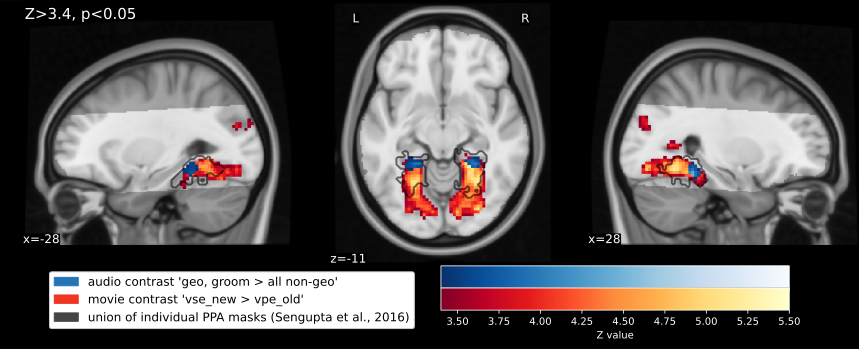
\includegraphics[width=\linewidth]{figures/group-slices}
    \caption{Mixed-effects group-level (N=14) GLM results. Significant clusters
        (Z>3.4, p<.05 cluster-corrected) are overlaid on the MNI152 T1-weighted
        head template (gray).
        Light gray: The audio-description's field-of-view
        (cf. \citep{hanke2014audiomovie}).
        Black: outline of overlapping individual PPA ROIs
        \citep{sengupta2016extension}.
        The results of audio-description's primary $t$-contrast (blue) that
        compares geometry-related nouns spoken by the narrator to non-spatial
        nouns (\texttt{geo, groom} > all non-spatial
        categories)
        are overlaid over the movie's primary $t$-contrast (blue) that compares
        cuts to a new setting with cuts to a familiar perspective
        (\texttt{vse\_new > vpe\_old}).
        }
    \label{fig:group-slices}
\end{figure*}


\begin{table*}[h!]
\caption{Significant clusters (z-threshold Z>3.4; p<.05 cluster-corrected)
    of the primary $t$-contrast for the audio-visual movie comparing cuts to a
    setting that was not depicted before to a recurring setting
    (\texttt{vse\_new > vpe\_old}).
    Clusters sorted by voxel size.
    The first brain structure given contains the voxel with the maximum Z-Value,
    followed by brain structures from posterior to anterior, and partially
    covered areas (l. = left; r. = right; c. = cortex; g. = gyrus).}
\label{tab:res-av-group1}
\begin{tabular}{rrrrrrrrrp{3cm}}
\toprule
& & & \multicolumn{3}{r}{max location (MNI)} & \multicolumn{3}{r}{center of gravity (MNI)} &
\\ \cmidrule{4-6} \cmidrule{7-9}
voxels & $p_{corr.}$ & Z-max & x & y & z  & x & y & z & structure \\
\midrule
3003 & 0 & 5.31 & 22.5 & -45.5 & -12 & 4.53 & -63.3 & -3.72 & r. lingual g.; r.
cuneal c., intracalcarine c., bilaterally occipital fusiform g., precuneus,temporal fusiform c., posterior parahippocampal c.  \\
154 & 0.000000656 & 4.46 & -35 & -83 & 28 & -32.8 & -86.2 & 21.4 & l. superior lateral occipital c. \\
121 & 0.00000769 & 4.65 & 25 & -80.5 & 25.5 & 23.7 & -83.8 & 25.4 & r. superior lateral occipital cortex \\
\bottomrule
\end{tabular}
\end{table*}


% table group results primary AD contrast
\begin{table*}[h!]
    \caption{Significant clusters (z-threshold Z>3.4; p<.05 cluster-corrected)
        of the primary $t$-contrast for the audio-description comparing
        geometry-related nouns to non geometry-related nouns spoken by the
        audio-description's narrator (\texttt{geo, groom > all non-geo}).
        Clusters sorted by voxel size.
    The first brain structure given contains the voxel with the maximum Z-Value,
followed by brain structures from posterior to anterior, and partially covered
areas (l. = left; r. = right; c. = cortex; g. = gyrus).}
    \label{tab:res-ao-group1}
\begin{tabular}{rrrrrrrrrp{3cm}}
\toprule
& & & \multicolumn{3}{r}{max location (MNI)} & \multicolumn{3}{r}{center of gravity (MNI)} &
\\ \cmidrule{4-6} \cmidrule{7-9}
voxels & $p_{corr.}$ & Z-max & x & y & z  & x & y & z & structure \\
\midrule
188 & 0.0000000596 & 4.48 & -17.5 & -65.5 & 25.5 & -14.7 & -59.1 & 15.2 & l. precuneus \\
164 & 0.000000238 & 4.47 & 17.5 & -58 & 23 & 15.6 & -55.6 & 16 & r. precuneus; \\
83 & 0.000128 & 4.48 & 27.5 & -43 & -17 & 27.2 & -41.1 & -14 & r. temporal (occipital) fusiform c.; posterior parahippocampal g. \\
73 & 0.000318 & 3.93 & -22.5 & -43 & -12 & -23.9 & -43.6 & -11.2 & l. lingual g.; temporal (occipital) fusiform g., posterior parahippocampal c. \\
63 & 0.000824 & 4.1 & 40 & -75.5 & 30.5 & 40.9 & -76.3 & 28.6 & r. superior lateral occipital c. \\
37 & 0.0129 & 4.24 & -37.5 & -78 & 33 & -38.4 & -79.5 & 28.9 & l. superior lateral occipital c. \\
\bottomrule
\end{tabular}
\end{table*}


% results in detail voxels of significant clusters in PPA ROI (and RSC
% liberally)
% sub-01 (m): PPA (l/r), AD (l/r), AV (-/r); RSC: AD (l/r), AV (-/-)
% sub-02 (m): PPA (l/r), AD (-/-), AV (l/-); RSC: AD (-/-), AV (-/-)
% sub-03 (f): PPA (l/r), AD (-/-), AV (-/r); RSC: AD (-/-), AV (-/-)
% sub-04 (f): PPA (-/r), AD (l/r), AV (-/r); RSC: AD (l/r), AV (-/-) !
% sub-05 (m): PPA (l/r), AD (-/-), AV (-/-); RSC: AD (-/-), AV (-/-)
% sub-06 (m): PPA (l/r), AD (l/r), AV (-/-); RSC: AD (l/-), AV (-/-)
% sub-09 (m): PPA (l/r), AD (l/-), AV (l/r); RSC: AD (l/r), AV (l/r)
% sub-14 (f): PPA (l/r), AD (l/r), AV (-/r); RSC: AD (l/r), AV (-/-)
% sub-15 (m): PPA (l/r), AD (l/r), AV (-/r); RSC: AD (l/r), AV (l/r)
% sub-16 (m): PPA (l/r), AD (l/r), AV (l/r); RSC: AD (l/r), AV (l/-)
% sub-17 (m): PPA (l/r), AD (l/r), AV (l/r); RSC: AD (l/r), AV (l/r)
% sub-18 (m): PPA (l/r), AD (l/r), AV (l/r); RSC: AD (l/r), AV (-/r)
% sub-19 (f): PPA (l/r), AD (l/r), AV (-/r); RSC: AD (l/r), AV (l/r)
% sub-20 (f): PPA (-/r), AD (-/-), AV (l/r); RSC: AD (-/-), AV (-/-)

% intro
Third, we investigated result from both naturalistic paradigms on the level of
individual subjects to ensure that the group results are not just a by-product
of the averaging process.
% AD is the real shit
Focussing on the AD stimulus, we hypothesize[d] that an exclusively auditory
stimulus can/could localize the PPA in individual subjects and thus
possibly substitute a visual paradigm [using blocks of pictures].

\todo[inline]{if we report procedure of Sengupta as detailed as it is now in the
following paragraph (imo it's too long), we probably need to explain the
differences between strict, relaxed, simple set in more detail in the method
section}
% Sengupta et al., 2016
The visual localizer experiment \citep{sengupta2016extension} yielded bilateral
[parahippocampal] clusters in 12 of 14 subjects and an unilateral right clusters
in two subjects (sub-04, sub-20).
% Sengupta: 1 of 3
Individual PPAs were assessed by visually inspecting thresholded $z$-maps
(Z>1.64, p<.05 cluster corrected) of three different $t$-contrasts
(\textit{strict}, \textit{relaxed}, and \textit{simple} stimulus set, cf.
\citep{sengupta2016extension}).
% procedure a)
Starting with the most conservative contrast (\textit{strict} set) and a
threshold of t = 2.5, we looked for clusters with at least 20 voxels (using
AFNI).
% procedure b)
We titrated [?] the threshold in the range of [2, 3] until we found an isolated
cluster for the PPA.
% Sengupta: procedure b)
If a cluster was not found or not isolated, we used a contrast from the
\textit{relaxed} set, or finally the \textit{simple} \todo{not used in any VP
for PPA}set, and repeated the process until we found a cluster that matched the
expected anatomical location based on literature \citep{epstein1998ppa}.

% one contrast to localize them all; "...and Z>3.4 for all"
Contrary to \citep{sengupta2016extension}, we used the same contrast of each
naturalistic stimulus and the same threshold for all subjects (Z>2.3, p<.05
cluster-corrected for the analysis in subject-space; Z>3.4, p<.05 for the
analysis in group-space).
% subject space -> NeuroVault
Results of the analyses that were performed in subject-space can be found in the
accompanying dataset. \todo{Neurovault does not like unstandardized spaces}
% here report in group space
For better comparisons of subjects, we here report results from the analyses
performed in group space.
% ref to figure
Figure \ref{fig:subs-thresh-ppa} depicts thresholded $z$-maps of the primary AV
and AD $t$-contrast, and the outline of overlapped, individual PPAs
\citep{sengupta2016extension}.
% MNI space
The $z$-maps and PPA outline are overlayed on the co-registered MNI152 template.
% one slice to show them all
Transversal slice of z=-11 was chosen as it depicts [at least some] voxels of
significant clusters in almost all subjects.

% AV
Results of the primary AV contrast yielded bilateral clusters in five subjects,
a unilateral right cluster in six subjects (of which one subjects yielded a
unilateral cluster in the visual localizer), and a unilateral left cluster in
one subject.
% difference to dedicated localizer
We find homologous clusters in sub-20, whereas the dedicated visual localizer
yielded only one cluster in the right hemisphere.

% report here in group
Results of the primary AD contrast yielded bilateral clusters in nine subjects
that are within or overlapping with the individual PPA.
% subj-04
In sub-04, two homologous clusters are apparent, whereas the dedicated localizer
(and AV stimulus) yielded only one cluster in the right hemisphere.
% sub-09
In sub-09 the analysis yielded one cluster in the left-hemispheric PPA.


\begin{figure*}[h!]
\centering
    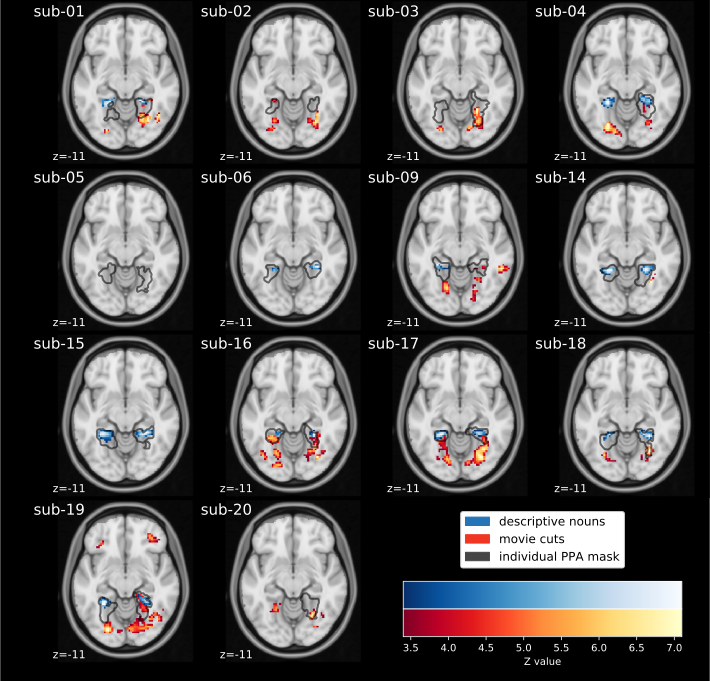
\includegraphics[width=\linewidth]{figures/subs-thresh-ppa}
    \caption{Fixed-effects individual-level GLM results (Z>3.4, p<.05
        cluster-corrected).
        Individual brains are aligned via non-linear
        transformation to a study-specific T2* group template that is
        co-registered to the MNI152 template with an affine transformation (12
        degrees of freedom).
        The results of audio-description's primary
        $t$-contrast (blue) that compares geometry-related nouns to non
        geometry-related nouns spoken by the audio-description's narrator
        (\texttt{geo, groom > all non-geo}) are overlaid over the movie's
        primary $t$-contrast (blue) that compares cuts to new setting with cuts
        to a familiar perspective (\texttt{vse\_new > vpe\_old}).
        Black:
        outline of subject-specific PPA ROIs.
        Light gray: The
        audio-description's field-of-view (cf. \citep{hanke2014audiomovie}).
        To facilitate comparisons across subjects, we chose the same horizontal
        slice (x=-11) for all subjects as this slice depicts voxels of
        significant clusters in almost all subjects.
        The figure does not show voxels of the left cluster of the AV stimulus
        in sub-09 and sub-18, and voxels of right cluster of the AV stimulus in
        sub-15.}
    \label{fig:subs-thresh-ppa}
\end{figure*}

\todo[inline]{BA-plots only shortly mentioned now}
% Bland-Altman-Plots
To better depict the agreement and difference between the results of the visual
localizer and the primary AD contrast, we created a Bland-Altman-Plot for every
subject (see ).
% what it depicts
Each subplot of Figure \ref{fig:bland-altman} visualizes the mean value and
difference (localizer minus AD) of two spatially corresponding voxels in the
unthresholded $z$-maps.
% top KDE plot
A shift of the distribution to voxels with a mean above zero can be seen the
further we constrain voxels to the individual PPA (see KDE plot for the x-axis).
% right KDE plot
Values above the horizontal line depict voxels that show a higher $z$-value in
the dedicated localizer, values below the horizontal line depict voxels that
show higher $z$-value in the AD stimulus.

\begin{figure*}[h!]
\centering
    \includegraphics[scale=0.27]{figures/subjs_bland-altman.png}
    \caption{Bland-Altman-Plots for individual subjects.
    The x-axes show the means of two spatially corresponding voxels in the
    unthresholded $z$-map of the audio-description's primary contrast and
    unthresholded $z$-map of the visual localizer (KDE plot on the top).
    The y-axes show the difference of two voxels (localizer minus
    audio-description; KDE plot on the right).
    The overlays depict voxels spatially constrained to the
    temporal and occipital cortex (gray; based on the probabilistic Jülich
    Histological Atlas \citep{eickhoff2005toolbox, eickhoff2007assignment}),
    PPA overlap of all subjects (blue),
    and individual PPA(s) (red).}
    \label{fig:bland-altman}
\end{figure*}


\subsection{Robustness of group results across contrasts}

% unthresholded $z$-maps of all contrasts on a group level:
% \href{https://neurovault.org/collections/KADGMGVZ/}{NeuroVault}.

\todo[inline]{I tried to keep following part concise but detailed; individual
contrasts are given but as numbers}

% AV PPA contrasts
% 1 PPA (l/r); RSC (l/r), LOC (l/r), VisC (l/r),
% intracalcarine, cuneal, ling.c
% 2 PPA (l/r); RSC (-/-), LOC (l/r), VisC (-/-)
% 3 PPA (l/r); RSC (-/-), LOC (-/-), VisC (-/r), occ. fusisf. g.
% 4 PPA (l/r); RSC (l/r), LOC (l/r), VisC (-/-), lingual g., occ. fusif. g.
% 5 PPA (l/r); RSC (l/r), LOC (l/r), VisC (-/-), occ. fusif. g.

% AV
In order to test the robustness of our findings, we created four additional
$t$-contrasts for the AV stimulus (see Table \ref{tab:av-contrasts}) to be
investigated on a group level.
% results: PPA; biggest overlap in posterior part of PPA group overlap  =
%temporal occipital fusiform cortex
All of the overall five AV contrasts yielded significant bilateral clusters that
overlap with the PPA group overlap (see Figure \ref{fig:stability-slices}).
% AD
For the AD stimulus, we created overall eight $t$-contrasts (see Table
\ref{tab:ao-contrasts}).
% results
All contrasts except contrast 7 (\texttt{se\_new}, \texttt{se\_old} >
non-spatial categories) and contrast 8 (\texttt{se\_new} > non-spatial
categories) yielded significant bilateral clusters in anterior regions of the
group PPA overlap (see Figure \ref{fig:stability-slices}).
% statement/answer
Results suggest that our findings are robust across differently designed
contrasts.\todo{concluding statement
often feels like interpretation}

% AD PPA contrasts
% 1 PPA (l/r); RSC (l/r), LOC (l/r)
% 2 PPA (l/r); RSC (l/r), LOC (l/r), r. sup.temp.C., r.fr.pole; putamen; etc
% 3 PPA (l/r); RSC (l/r), LOC (l/r),l&r sup.temp.C., anterior cing., paracing.
% 4 PPA (l/r); RSC (l/r), LOC (l/r)
% 5 PPA (l/r); RSC (l/r), LOC (-/-)
% 6 PPA (l/r); RSC (l/r), LOC (l/-), l&r sup.temp.C.; medial pref. c., precun
% 7 PPA (-/-); RSC (l/r), LOC (l/-), l&r sup.temp.C.; left frontal pole
% 8 PPA (-/-); RSC (-/-), LOC (-/-)

% AD
Reliably across the five contrasts of the AV stimulus, we find bilaterally
significant clusters also in the ventral precuneal cortex and posterior
cingulate gyrus (i.e. restrosplenial region; contrasts 1, 4, 5) and lateral
occipital cortex (contrasts 1, 2, 4, 5).
% AD; LOC: AV cluster are more medial, AD clusters are more lateral
Across the five contrasts of the AD stimulus, we find bilaterally
significant clusters in the ventral precuneus (all except contrasts 8), lateral
occipital cortex (bilateral in contrasts 1 to 4; unilateral in contrasts 6 and
7), and superior temporal cortices (bilateral in contrasts 3, 6, 7; unilateral
right in contrast 2).

% non-systematic
Lastly, some contrasts of the AD stimulus yielded signficant clusters in regions
that were not statistically signficant in three or more contrasts.
%
Contrast 2 yielded clusters in the anterior cingulate gyrus
(bilateral), right frontal pole, right frontal medial cortex, and right
putamen.
%
Contrast 3 shows clusters in the anterior cingulate gyrus (bilateral), left
frontal pole, and left insular.
%
Contrast 7 shows clusters in the left frontal pole and left frontal operculum
[border to triangularis], left insular.
%
Contrast 6 shows one additional cluster in the right medial frontal cortex.


\begin{figure*}[h!]
\centering
    \includegraphics[width=\linewidth]{figures/stability-slices}
    \caption{Overlap of significant clusters (Z>3.4; p<.05, cluster corrected)
        The audio-description's contrasts 1-8 (blue; \ref{tab:ao-contrasts})
        are overlaid over the audio-visual movie's contrasts 1-5 (red;
        \ref{tab:av-contrasts}).
        Cluster are overlaid on top of the MNI152 T1-weighted head template
        (gray).
        Black: outline of overlapping individual PPA ROIs.
        Light gray: The audio-description's field-of-view (cf.
        \citep{hanke2014audiomovie}).
        The figure shows that some contrasts yielded significant clusters
        also in the lateral temporal and prefrontal cortex.
        }
    \label{fig:stability-slices}
\end{figure*}


\subsection{control contrasts}

% ---------- AV control contrasts ----------
% 6 nothing
% 7 nothing
% 8 nothing
% 9 nothing
%10 se_new > se_old (nouns but in AV stimulus):
% LOC (l/r) right PPA, bilateral sup. lat. occ. c., sup. parietal lobe (right)

% ---------- AD control contrasts ----------
% 9 PPA (-/-); RSC (-/r), LOC (-/-), left pars triangularis
%10 PPA (-/-); RSC (-/-), LOC (-/-)
%11 PPA (-/-); RSC (-/-), LOC (-/-),
%12 PPA (-/-); RSC (-/-), LOC (-/-), right posterior hippocampus
%13 PPA (-/-); RSC (-/-), LOC (-/-)

\todo[inline]{there is no table/figure for negative control contrasts; we could
add a reference to NeuroVault (here again) or point to the dataset}

% intro
Lastly, we implemented five contrasts for every stimulus for the purpose of
negative control.
% AV: no_cut > x
In the analysis of the AV data, none of the contrasts that compared the ``no cut
condition''  to a movie cut category (contrasts 6, 7, 8, 9) yielded significant
clusters.
% AV using nouns
The contrast that used the narrator's nouns but in the AV stimulus (se\_new >
se\_old) yielded a significant cluster in the right PPA and bilateral clusters
in the superior lateral occipital cortices (the right hemispheric cluster
extending into the superior parietal cortex).

% AD stimulus
In the analysis of the AD data, we created control contrasts based on events of
the annotated movie cuts (cf. Table \ref{tab:ao-contrasts})
% contrast 9
Contrast 9 (vse\_new > pe\_old) revealed one significant cluster in the left
inferior prefrontal cortex (pars triangularis) and right ventral
precuneus/posterior cingulate gyrus.
% contrast 12
Contrast 12 (\texttt{vse\_new} > \texttt{vse\_old}, \texttt{vpe\_old}) revealed
one cluster in the right posterior hippocampus. \todo{definitively hippocampus,
dorsally of PPA}




\section{Discussion}

% Discussion: explains how results fill gap identified in intro

% typically done by recapitulating the results, discussing limitations, and then
% revealing how the central contribution may catalyze future
% progress

% provides caveats to the interpretation describes how the paper
% advances the field by providing new opportunities

\todo[inline]{SE: sauber differenzieren zwischen "Lokalisation der PPA" und
    "Antwortverhalten einer vorab definierten PPA". Ich habe den Eindruck, dass
Du oft das erste machst es aber als das zweite beschreibst; COH: ??? we do
whole-brain analysies, so probably ``localization'', }

% previous studies
Previous studies reported bilaterally increased hemodynamic activity in the PPA
when participants were watching static pictures of landscape compared to
pictures of faces or objects (e.g. \citep{epstein1998ppa,
epstein1999parahippocampal}) whereas one study using spoken sentences reported
mixed results \citep{aziz2008modulation}.
% current study: similar
In line with previous studies, we use here also operationalize spatial
perception via general linear model (GLM) $t$-contrasts in two naturalistic
stimuli.
% current study: dissimilar
Contrary to previous studies, our current approach is not based on
carefully designed sets of stimuli but based on annotated stimulus features
incidentially occurring in an audio-visual movie and its audio-description.
% group AV
On a group level, whole brain-analysis results for the movie stimulus show
signifcantly increased hemodynamic activity spatially overlapping with a
traditionally localized PPA but also extending into earlier visual cortices.
% group AD
Results for the audio-description stimulus reveal significant activation
restricted to the anterior part of the PPA.
% individual level
On an individual level, results of the audio-description show significant
bilateral clusters in the anterior PPA of nine subjects and significant
unilateral clusters in two subjects.
% meaning 1
Results suggest that increased activation in the PPA during the perception of
static pictures generalizes to the perception of spatial information embedded in
a movie and an exclusively auditory stimulus.
% meaning 2
Our results provide further evidence that the PPA can be divided into functional
subregions. An auditory narrative might substitute a visual paradigm to localize
the PPAs anterior part in visually impaired subjects.


\subsection{PPA; AV \& AD; group \& individuals}

\todo[inline]{SE: VIS vs AV vs AD: Wer liefert was über die PPA. Dieser
Vergleich bzw. die Diskussion über Gemeinsamkeiten \& Unterschiede fehlt mir
etwas}

\subsubsection{AV: group}


% intro
First, we analyzed data from the movie stimulus offering ecologically more valid
but still visual stimulation.
%
An early study \citep{bartels2004mapping} that manually annotated the content
(color, faces, language, and human bodies) of movie frames found that
specialization of functional areas is preserved during movie watching.
%
Contrary to \citep{bartels2004mapping}, we categorized the frames after movie
cuts independent of the frames' content.\todo{PPA in
    \citep{hasson2004intersubject} but do reverse ISC}
% hypo
Despite this ``adventurous'' / ad hoc approach, we hypothesized that
[confounding variables could/would average out and] our whole-brain analyses
would lead to significant clusters in the PPA.
% results
Group results of the AV stimulus' primary contrast yielded a clusters that span
the group overlap of individual PPA ROIs from anterior to posterior.
% difference in location/size to AD and VIS
The cluster also extends into medial regions (dorsal precuneus and dorsal
posterior cingulate cortices), and into more posterior regions (occipital
fusiform gyrus and intracalcarine cortex) bilaterally.
% confound of higher perception
The larger extension into more posterior, primary visual areas can be attributed
to the fact that we averaged the content of individual frames after a cut and
did not control for confounding features like depicted faces or objects or
attentional focus of subjects.
%
\todo[inline]{bigger size of clusters is not surprising;  imo still impressive
low amount of random clusters in the brain (and not one third of brain
significant); Clusters in Bartels (2004) are actually kinda big, too;)}
%
Noteworthy, we here exploited a confound in the stimulus structure induced by
cinematographic tendencies (cf. method section;
% a)
a) movies tend to establish the setting and the spatial relationships within a
setting at the beginning of a movie;
% b)
b) the field sizes of movie shots tend to decrease when switching back to
already established settings
% c)
c) shots within a recurring locale or setting tend to shift to depicting persons
and objects \citep{brown2012cinematography, mercado2011filmmakers}.
% interpretation
-> concluding statement?
% shortcomings
Since the capability to isolate clusters or networks correlating with specific
perceptual (or cognitive) processes is influenced by the amount of annotated
stimulus features further studies focusing on visual perception should annotate
and model visual features of naturalistic stimuli more rigorously.
% solution
Future studies that aim to use a movie to localize different visual areas should
extensively annotate the content of frames (e.g. using the open-source solution
``Pliers'' for feature extraction from a visual naturalistic stimulus;
\citep{mcnamara2017developing}) and record the subject's visual attention via
eye-tracking.

\todo[inline]{Nevertheless: that this simple approach works actually suprisingly
well; shows that a lot of confounds average out, since we clusters are not super
big or all over the brain (and that across contrasts)}

\todo[inline]{on the other hand: movies are nice but have idiosyncrasies; so,
maybe you should be aware of these idiosyncrasies (and control for it) in case
you wanna use movies for research}

% summary: nevertheless
\todo[inline]{Summary: so, yes, what is the main message of this
``cross-modal-control-movie-thing''?? cf. intro: ``works'' but clusters more
widespread}


\subsubsection{AD: group}

\todo[inline]{Aziz: reduced activity only in left PPA, and only for famous
places vs famous faces; I think they ran their f-test on the average of the PPA
voxels! anyway: their analysis is complicated, yet not sophisticated}

% intro
Second, we analyzed data from the audio-description.
% hypothesis
Encouraged by \citep{aziz2008modulation}, we also hypothesized that spatial
information embedded in an exclusively auditory stimulus would correlate with
increased hemodynamic activity in the PPA.
% results
Group results of the AD stimulus' primary contrast yielded spatially concise
clusters in the anterior part of the PPA group overlap that we gained from a
visual localizer experiment \citep{sengupta2016extension}.
% diff to Aziz (2008)
Unlike \citep{aziz2008modulation} who modeled events from on- to offset of
sentences (describing unknown and famous places and faces), we modeled events
from on- to offset of single words (that indicats the visual content to the
listener).
% conclusion
\citep{aziz2008modulation} found significantly increased activity in only the
left PPA and only for sentences describing famous places compared to famous
faces.\todo{averaged across voxels in PPA/FFA defined by localizer}
%
Contrary, our group results suggest that auditory spatial information
compared to non-spatial information correlates with bilaterally increased
activation in its anterior.\todo{any concluding statement?}

% previous studies: no task
Usually studies that use small sets of experimentally controlled stimuli also
employ a task to keep subjects attentive to the stimuli.
% but: Epstein (1998)
Nevertheless, one early block-design study \citep{epstein1998ppa} compared
results from a paradigm that employed a (perceptual) judgment task of static
pictures to the same paradigm but without that task.
% results during no task
Hemodynamic activity was less but still significantly increased when
participants had no task to keep them alert and attentive to the stimuli.
% we have no task neither
Our paradigm is similar in that sense that our participants had no behavioral or
cognitive task (e.g. forming a mental image of the stimuli; cf.
\citep{ocraven2000mental})  but just had to ``enjoy the audio-description''.
% but still: we are different
Our paradigm still differs from \citep{epstein1998ppa} because the modeled
stimulus features were incidentally embedded in a continuous stream of auditory
information preventing participants from making assumptions about the
investigated perceptual process.
% concluding statement: kinda automatic process
Hence, current results from our paradigm also suggest that verbal spatial
information is processed in the anterior PPA casually and does not [necessarily]
rely on [deliberately] paying attention to verbal spatial information.


\subsubsection{AD: individuals}

\todo[inline]{how to discuss Bland-Altman-Plots???; dunno if this is meaningful:
z-scores in the anterior part of PPA are higher in AD contrasts than in contrast
of localizer}

\todo[inline]{We hypothesize[d] that an exclusively auditory stimulus can/could
localize the PPA in individual subjects, and thus substitute a visual experiment
be which would be more practicable to assess brain functions in visually
impaired persons.}

%
Since the annotation of the narrator's voice allowed us to better/cleaner/nicer
operationalize spatial perception than the movie's annotation, we here
hypothesized
% AD stimulus

% intro
To test if an auditory narrative could substitute a visual localizer experiment,
we also examined the results of the primary AD contrast on the level of
individual subjects.
% results of dedicated localizer
The visual localizer \citep{sengupta2016extension} revealed bilateral ROIs in 12
of 14 subjects and a unilateral right ROI in two subjects (sub-04, sub-20).
% in the current study
The audio-description's primary contrast yielded significant bilateral clusters
in 9 of 14 subjects (of which sub-04 shows just right-lateralized PPA ROI) and a
unilateral significant cluster in one subject.
%
Whereas \citep{sengupta2016extension} chose the subjectively ``best fitting
$z$-threshold in a subject's unthresholded $z$-map by visual judgment, we used a
``one threshold fits all approach`` (Z>3.4, p<.05 cluster-corrected).
% group vs individual
Results on an individual level reveal that significant cluster are located in
the anterior part of individual PPA ROIs. Thus, the pattern that was revealed on
a group level is not just a by-product of the averaging process but can reliably
be found in individual study participants.
% conclusion
Lastly, our exploratory analyses suggest that a naturalistic auditory stimulus
is in principle suitable to localize (the anterior part) of a higher-level
visual area in the majority of subjects.
% chose the best contrast in the future
Similarly to \citep{sengupta2016extension} that chose the ``best'' of three
alternative contrasts (strict, relaxed, or simple contrast), future studies that
aim for individual diagnostics / ROI localization should also test more than one
contrast to gain the ``best'' individual ROIs.\todo{``best'' sounds pretty
shitty}

\todo[inline]{discussion of individual differences? what do the results
suggest? Differences in alertness, attention to spatial information,
predisposition? ``capability'' to process auditory spatial information?}

\todo[inline]{individual ``preference'' to pay attention to
spatial infos (which contradicts statement above that attention is not a
prerequisite)}

\subsubsection{AD: shortcoming}

% optimal stimulus type in vision
In the visual domain, landscapes and not pictures of landmarks or buildings are
considered to be the ``optimal'' stimulus type (cf. Epstein (1998, 1999, 2003,
2008).\todo{check references}
% cateogries in primary contrasts
In the current study's primary contrast, we compared verbal hints about
landmarks ((\texttt{geo}; often buildings or other single aspects of a whole
scene) and elements defining the geometry of a room or locale (\texttt{groom})
to non-spatial hints.
% we did not choose se\_new and se\_old
We did not choose the categories that contained switches from one setting to
another (\texttt{se\_new} and \texttt{se\_old}) which one might assume to
contain the auditory equivalent to the ``optimal'' visual stimulus type.
% why not se\_new or se\_old
The categories \texttt{se\_new} and \texttt{se\_old} were actually
heterogeneous: they rarely contained whole and thus a vague verbal descriptions
of landscapes (e.g. ``in a football stadium'', ``Forrest is running through the
jungle'') but mostly landmarks or buildings, and also non-spatial hints (e.g.
``Jenny as a teenager``).
% further studies
Given that humans can identify the gist of a rich visual scene within the
duration of a single fixation \citep{henderson2003human} further studies might
investigate if categories of holistic but vague verbal descriptions of
landscapes correlate with differential hemodynamic activity in the PPA compared
to more concrete spatial hints.
% future studies
Hence, future studies might investigate if a homogenous category of wholistic
but vague verbal descriptions (e.g. ``a mountain landscape'') compared to a
homogenous categories of more specific verbal descriptions of landmarks (e.g.
``a beacon'') or houses (e.g. ``farmhouse'', ``apartment building'') lead to
different levels of hemodynamic activity.


\subsection{Robust (results) across contrasts}

\todo[inline]{SE: Bei Ergebnissen \& Diskussionen zu Stability fehlt mir
irgendwie immer der Kontext, wie sich die Kontraste denn unterschieden haben und
welche davon z.B. im Ergebnis wo von den anderen abgewichen haben. Das würde ja
wichtige Hinweise geben; COH: indeed very interesting but discussing that will
let the paper get way out of hand}

\todo[inline]{yeah, we have shortcomings but, look, we have a pattern of
spatially restricted clusters across contrasts (and stimuli)}

% more than just one contrast
For both naturalistic stimuli, we computed several $t$-contrasts that differed
in the contrasted categories of stimulus features and the amount of available
data to test the robustness of our findings.
% why we did a couple of contrasts
m.a.w.: For both stimuli we created several contrasts that varied the amount of
events available for the analysis and how well the annotated events within
categories on average matched the stimulus type that we assumed to be
preferentially processed in the PPA.

\subsubsection{PPA}

% PPA AV
Regarding contrasts of the AV stimulus, all five contrasts show significant
bilateral clusters in the PPA but also extending into more posterior brain
regions
\todo[inline]{cf. discussed shortcomings}

% PPA AD
Regarding contrasts of the AD stimulus, six of eight contrasts show significant
bilateral clusters in the anterior part of the group PPA overlap.

% results indicate robustness
Thus, the results of the additional contrasts indicate that our findings are
robust across contrasts do not depend on the design of one specific
contrasts.

% but
Nevertheless, results are still influenced by [sensitive to] the amount of
available data and how well the feature space is modeled.
% example
For example, contrast 8 of the AD stimulus (\texttt{se\_new} > texttt{se\_old})
that used the most heterogeneous categories comprising the least amount of
events yielded neither a significant cluster in the right-hemispheric nor
left-hemispheric PPA.
% concluding statement
Hence, investigators using model-driven analyses have to consider how many
events a stimulus to be chosen may provide and how homogeneous the events to be
averaged might be.


\subsubsection{anterior vs. posterior PPA}

\todo[inline]{the mother of total confusion: Aminoff shifts the PPA along the
    anterior-poster axis depending on publication;
    in Aminoff (2007, 2013):
    anterior PPA = spatial associations,
    region anterior to (!) PPA = non-spatial associations;
    in Aminoff (2015):
    posterior PPA = spatial associations,
    anterior PPA = non-spatial associations;
    hence: complete bullshit;
    ignore Aminoff (2015) due to various reasons}

% intro
Results of the AD contrasts consistently yielded significant clusters spatially
constrained to the anterior part of the PPA group overlap [and to the anterior
part of significant clusters of the AV contrasts].
% PPA might have submodules
Previous studies provide evidence that the PPA can be devided into functionally
subregions that might process different stimulus features [during visual scene
perception].
% posterior: functionality
The posterior PPA (pPPA) is functionally more responsive than the anterior PPA
(aPPA) to low-level features of scenes or (abstract) objects
\citep{baldassano2013differential, nasr2014thinking,
rajimehr2011parahippocampal}.
% anterior cIPL is defined using the Eickhoff–Zilles PGp probabilistic
% cytoarchitectonic map
The aPPA is functionally more responsive than pPPA to high-level features of
scenes (e.g. real-word size \citep{park2015parametric}; a scene's abstract
identity/category \citep{marchette2015outside, watson2016patterns}) and objects
(e.g. spatial contextual associations \citep{aminoff2007parahippocampal,
aminoff2013role}).
% connectivity
Moreover, pPPA and aPPA show differences in connectivity profiles.
% posterior
The pPPA is more strongly functionally connected to the occipital visual cortex
than the aPPA \citep{baldassano2013differential, baldassano2016two}.
% including lateral occipital cortex (LOC) and transverse occipital sulcus (TOS)
% anterior
The aPPA is more strongly functionally connected to portions of the default mode
network, including caudal inferior parietal lobe (cIPL), the restrosplenial
complex (RSC), medial PFC and the lateral surface of the anterior temporal lobe
\citep{baldassano2013differential, baldassano2016two}.
% conclusion: subregions
According to the hypothesis by \citep{baldassano2013differential} the PPA
consists of subregions that activate selectively to scenes and ``cooperate to
build a complete representation of a scene''.
% Their distinct connectivity properties do suggest that each may be involved in
% specific aspects of visual and cognitive processing involved in the
% overarching goal of scene understanding \citep{baldassano2013differential}.
% The fact that anterior PPA had a lower sensitivity to our abstract object
% stimuli does not necessarily imply that this region does not use object
% information \citep{baldassano2013differential}. Previous work has shown that
% PPA responds to objects that have spatial associations [Aminoff et al. 2007],
% are space-defining [Mullally and Maguire 2011], and are
% navigationally-relevant [Janzen and Van Turennout 2004]. These types of
% responses require spatial memory and cannot be based purely on visual features
% like object shape. \citep{baldassano2013differential}.
Our results add further evidence that the PPA is not a homogeneous area but can
be devided into functionally subregions.
% pPPA
Results of your study suggest that the pPPA is more concerned with visual
aspects of spatial information as exclusively inherent in visual stimuli like
pictures or movies.
% aPPA
The aPPA might be more concerned with non-visual aspects of spatial information
(e.g. spatial contextual information \citep{aminoff2013role,
aminoff2015associative, baumann2016functional}) inherent in both visual and
verbal stimuli.


\subsubsection{retrosplenial cortex (RSC)}

\todo[inline]{SE: RSC etc: Irgendwie waren die bis zu Diskussion eher ein
afterthought. Daher etwas überraschend, vielleicht in Einleitung und Results
schon mehr bringen; COH: afterthought, for sure; It was highly probable that RSC
would show up but it wasn't aim of the study (had no ROIs for it anyway); imo
this is an issue of ``nice story telling'' vs. HARKing}

% but RSC
Apart from the PPA, we find significantly increased activity in the
retrosplenial cortex (RSC) consistently across contrasts of both stimuli (AD
stimulus: 7 contrasts; AV stimulus: 3 contrasts).
% location functionally defined
The RSC as a scene-selective region is not necessarily spatially congruent with
the anatomically defined retrosplenial cortex [26] (BA 29 and 30)
\citep{epstein2008parahippocampal} but functionally defined as the posterior
medial region that exhibits increased hemodynamic activity to visual scenes and
during mental imagination trough familiar environments [8]
\citep{epstein2008parahippocampal}.
% location
This functionally defined RSC is located in the retrosplenial cortex, and
posterior cingulate region (BA 23 and 31) [51–56], near to the point where the
calcarine sulcus joins the parietal-occipital sulcus
\citep{epstein2008parahippocampal}.

% discussion of what the RSC does
interpretation cf.:
\begin{itemize}
    \item \citep{chrastil2018heterogeneity}
    \item \citep{vann2009what}
    \item \citep{silson2019posterior}
    \item \citep{baldassano2016two}:
    \item RSC appears to be most directly involved in orienting the viewer to
    the structure of the environment (both within and beyond the borders of the
presented image) for the purpose of navigational planning; it encodes both
absolute location and facing direction [Vass and Epstein, 2013; Epstein and
Vass, 2014; Marchette et al., 2014], integrates across views presented in a
panoramic sequence [Park and Chun, 2009], and shows strong familiarity effects
[Epstein et al., 2007a,b].
\end{itemize}


\subsubsection{superior lateral occipital cortex (TOC / OPA?)}

\begin{itemize}
\item Bettencourt (2013). The Role of Transverse Occipital Sulcus in Scene
    Perception
\item Dilks, Kanwisher (2013). The Occipital Place Area Is Causally and
    Selectively Involved in Scene Perception
\item Nasr (2011). Scene-selective cortical regions in human and nonhuman
    primates
\item Dilks (2011). Mirror-image sensitivity and invariance in object \& scene
    processing
\item MacEvoy and Epstein (2007). Position selectivity in scene- and
    object-responsive
\item Grill-Spector (2003). The neural basis of object perception
\item Hasson (2003). Large-scale mirror-symmetry organization
\item Nakamura (2000). Functional delineation of the human occipito-temporal
    areas
\item \citep{baldassano2016two} regarding functional difference pPPA vs. OPA:
    The functional distinction is unclear.
    Previous work has speculated about the purpose of the apparent ventral and
    dorsal ``duplication'' of regions sensitive to large landmarks, proposing
    that it may be related to different output goals (e.g., action planning in
    OPA, object recognition in pPPA)[Konkle and Caramazza, 2013], or to
    different input connections (e.g., lower visual field processing in OPA,
    upper visual field processing in pPPA)[Kravitz et al., 2013; Silson et al.,
    2015].
    OPA and pPPA may also use information from different visual
    eccentricities: OPA processing less peripheral, relatively high-resolution
    environmental features. pPPA processing more peripheral, large-scale
    geometry, and context [Baldassano et al., 2016a]
\end{itemize}


\todo[inline]{in any case: the pattern PPA, RSC, LOC is a usual pattern in the
visual domain; here, it is the usual pattern across across AV and AD contrasts
-> hypothesis for auditory domain? future research and stuff?}

\subsubsection{not many random cluster}

\todo[inline]{makes sense because it goes full circle to general naturalistic
stimulus topic and makes transition to negative controls easier (which is
essentially also "natural stimuli, fuck yeah!}

% ``confounding'' clusters
Despite performing a whole brain analysis, we do not find many [random] clusters
in single contrasts or even systematically across contrasts that hamper the
interpretation of results.\todo{ouff\dots}
% AV: null results regarding attention and eye movements
For example in the AV results, we do not find significant clusters that could be
attributed to cognitive processes like attention or eye movements\todo{could
already already be mentioned in discussion of primary contrasts}


% AD: auditory cortices
Nevertheless, contrasts of the AD stimulus that compare (among others) verbal
hints of the change of a setting (\texttt{se\_new} or \texttt{se\_old}) to all
non-spatial categories (cf. contrasts 2, 3, 6, 7) show significant clusters in
(primary and secondary) auditory cortices.
% averaging vs. nuisance regressors
This suggests that variance correlating with lower level auditory processes was
not averaged out across trials and nuisance regressors did not capture enough
variance.\todo{ouf\dots}
% possible reason
Significant clusters in auditory cortices could be correlating with a possible
change of the soundscape when the narrator of the audio-description (or a cut in
the movie) switches to a another setting.
% concluding statement
Thus, investigators that use model-driven methods to investigate brain functions
using naturalistic stimuli should (extensively) annotate the stimulus material
and test for correlations among variables.

\subsubsection{random shower toughts}

Cuts probably correlate with change in soundscape; change in soundscape often
anticipates narrator (would lower detection power) or occurs in parallel with
narrator; cf. correlation of cuts to other setting (independent of familiarity)
with nouns that indicate a change of setting; cf. control contrasts [which
ones?]
% arnott hypothesis
We hypothesize that not just semantic information but also the mere changes of a
soundscape that indicate a setting's spatial layout could correlate with
increased activity in the PPA.
% arnott
\todo[inline]{e.g. arnott2008crinkling finds increased activations in PPA to
sounds made by objects (that reveil object's material/identity)}


\subsection{negative controls and cross-modal controls}

\todo[inline]{could be mentioned in a few sentences. But above topics a far too
much still; better embed somewhere above}

% AV: contrast with AV nouns
Compare Figure \ref{fig:reg-corr}: nouns that indicate a change to a new setting
are correlated  with cuts to a new setting (vse\_new; r$\approx$0.3; second
highest correlation of a verbal hint category with a cut category; AND: nouns
that indicate change to a familiar setting are somewhat correlated with cuts to
a familiar setting (se\_old; r$\approx$0.4; highest correlation of a verbal
category with a cut category).

% AD: correlation of these nouns with cuts
Compare Figure \ref{fig:reg-corr}: nouns that indicate change to a new setting
are correlated  with cuts to a new setting (vse\_new; r$\approx$0.3; second
highest correlation of a verbal hint category with a cut category.





\section{Conclusions}

\todo[inline]{SE: frage ich mich das beim Durchgehen: Warum ist der Fokus so
sehr auf Audiobook / AD, während AV doch eigentlich more natural and engaging
ist? COH: at the moment, the discussion is not tailored to the topic
``naturalistic stimulus as substitute to localizer'' as it is not and should not
be the main focus}

\todo[inline]{template has no section ``conclusion'' -> use the last paragraph}

% natural stimulation
Natural stimuli like movies \citep{eickhoff2020towards,
hasson2008neurocinematics, sonkusare2019naturalistic} or narratives
\citep{hamilton2018revolution, honey2012not, lerner2011topographic,
silbert2014coupled, wilson2008beyond} offer an easy to implement, (continuous,)
complex, immersive, task-free paradigm that more closely resembles our natural
dynamic environment than traditional experimental designs.

\begin{itemize}
\item We reuse public data for independent research question
\item GLM based on annotations to operationalize ``spatial perception''
\item Our results add evidence that model-driven analyses based in annotations
can be run on data from naturalistic stimuli to ``localize'' brain activity
correlating with specific perceptual processes.
\item ``localization performance'' relies on how well the model captures
different aspects of the stimuli's feature space.
\item PPA is functionally heterogenous region
\item a complex but naturally engaging auditory stimulus like an
audiobook might in principle be used as a non-visual localizer for a variety of
brain functions in subjects who are not willing or able to follow task
instructions during brain scanning [would state that explicitly in the summary
at the end].
\end{itemize}

% \citep{hanke2014audiomovie}: the AD stimulus leaves a much larger margin for
% inter-individual differences in imagining scenery. The AD stimulus limits the
% effect of an attentional focus on the selection of a subset of simultaneously
% occurring auditory events, in contrast to the selection of different parts of
% the visual field.


\subsection*{Code availability}
% wo kommt dieser Abschnitt hin?  how to write Code availability statement
% https://www.springernature.com/gp/authors/research-data-policy/data-availability-statements/12330880
\todo[inline]{provide supporting source code, and explaining how and where
others may access all data underlying the analysis} \emph{for all studies using
    custom code in the generation or processing of datasets, a statement must be
    included here, indicating whether and how the code can be accessed,
including any restrictions to access; include information on the versions of any
software used, if relevant, and any specific variables or parameters used to
generate, test, or process the current dataset. }

\section*{Acknowledgements}
% Text acknowledging non-author contributors. Acknowledgements should be brief, and should not include thanks to anonymous referees and editors, or effusive comments. Grant or contribution numbers may be acknowledged.
% Author contributions Please describe briefly the contributions of each author to this work on a separate line.
\emph{COH did this and that.
MH did this and that.
We are grateful to \href{www.florianschurz.de}{Florian Schurz} who initiated doing the annotation of the descriptive nouns, and performed the preliminary annotation of nouns.}

\section*{Competing financial interests}
\emph{A competing financial interests statement is required for all accepted
papers published in \emph{Scientific Data}. If none exist simply write,
``The author(s) declare no competing financial interests''.}

\section*{Figures Legends}
\emph{Figure should be referred to using a consistent numbering scheme through
the entire Data Descriptor. For initial submissions, authors may choose
to supply this document as a single PDF with embedded figures, but
separate figure image files must be provided for revisions and accepted
manuscripts. In most cases, a Data Descriptor should not contain more
than three figures, but more may be allowed when needed. We discourage
the inclusion of figures in the Supplementary Information \textendash{}
all key figures should be included here in the main Figure section.}

\emph{Figure legends begin with a brief title sentence for the whole figure
and continue with a short description of what is shown in each panel,
as well as explaining any symbols used. Legend must total no more
than 350 words, and may contain literature references.}

\section*{Tables}

\emph{Tables supporting the Data Descriptor. These can provide summary information
(sample numbers, demographics, etc.), but they should generally not
be used to present primary data (i.e. measurements). Tables containing
primary data should be submitted to an appropriate data repository.}

\emph{Tables may be provided within the \LaTeX{} document or as separate
files (tab-delimited text or Excel files). Legends, where needed,
should be included here. Generally, a Data Descriptor should have
fewer than ten Tables, but more may be allowed when needed. Tables
may be of any size, but only Tables which fit onto a single printed
page will be included in the PDF version of the article (up to a maximum
of three).}

{\small\bibliographystyle{unsrtnat}
\bibliography{references}}

%\begin{thebibliography}{1}
%\expandafter\ifx\csname url\endcsname\relax
%  \def\url#1{\texttt{#1}}\fi
%\expandafter\ifx\csname urlprefix\endcsname\relax\def\urlprefix{URL }\fi
%\providecommand{\bibinfo}[2]{#2}
%\providecommand{\eprint}[2][]{\url{#2}}
%
%\bibitem{cite1}
%\bibinfo{author}{Califano, A.}, \bibinfo{author}{Butte, A.~J.},
%  \bibinfo{author}{Friend, S.}, \bibinfo{author}{Ideker, T.} \&
%  \bibinfo{author}{Schadt, E.}
%\newblock \bibinfo{title}{{Leveraging models of cell regulation and GWAS data
%  in integrative network-based association studies}}.
%\newblock \emph{\bibinfo{journal}{Nature Genetics}}
%  \textbf{\bibinfo{volume}{44}}, \bibinfo{pages}{841--847}
%  (\bibinfo{year}{2012}).
%
%\bibitem{cite2}
%\bibinfo{author}{Wang, R.} \emph{et~al.}
%\newblock \bibinfo{title}{{PRIDE Inspector: a tool to visualize and validate MS
%  proteomics data.}}
%\newblock \emph{\bibinfo{journal}{Nature Biotechnology}}
%  \textbf{\bibinfo{volume}{30}}, \bibinfo{pages}{135--137}
%  (\bibinfo{year}{2012}).
%\end{thebibliography}

\section*{Data Citations}

Bibliographic information for the data records described in the manuscript.

1. Lastname1, Initial1., Lastname2, Initial2., ...\& LastnameN, InitialN. \emph{Repository name} Dataset accession number or DOI (YYYY).

\end{document}
\documentclass[english]{article}
